\documentclass[twoside,openleft,reqno,a4paper,final]{book}
%%% Remove the next two lines if you want the figures at their place
%\usepackage[figuresonly,nolists,nomarkers]{endfloat}
%\renewcommand{\processdelayedfloats}{}

\usepackage{soul}%strikeout \st


\usepackage[T1]{fontenc}
\usepackage[utf8]{inputenc}
\usepackage[version=4]{mhchem}
\usepackage{hyperref,booktabs,algpseudocode,algorithm,booktabs,titlesec,setspace,relsize}
\usepackage{natbib,amsmath,xcolor,graphicx,float,subcaption}
\usepackage[toc,page]{appendix}
\setcitestyle{square}


%\pagenumbering{roman}  http://www.markschenk.com/tensegrity/latexexplanation.html
 %A4 (210 mm x 297 mm)  https://tex.stackexchange.com/questions/20538/what-is-the-right-order-when-using-frontmatter-tableofcontents-mainmatter
%\addtolength{\textwidth}{12mm}%210
%\addtolength{\evensidemargin}{-4mm}
%\addtolength{\oddsidemargin}{-8mm}
%\addtolength{\textheight}{35mm}%297
\setlength{\parskip}{1.3ex plus 0.2ex minus 0.2ex}
\setlength{\parindent}{0pt}

\usepackage[bindingoffset=25mm, left=15mm, right=15mm,top=30mm, bottom=20mm]{geometry}
\usepackage{float}
\usepackage{fancyhdr}
\pagestyle{fancy}
\renewcommand{\chaptermark}[1]{\markboth{\thechapter~-~#1}{}}
 \fancyhf{}
  \fancyhead[LE]{\itshape   \thepage}
 \fancyhead[RE]{\itshape  \nouppercase{\rightmark}} %\nouppercase !
  \fancyhead[LO]{\itshape  \nouppercase{\leftmark }}%thechapter
 \fancyhead[RO]{\itshape  \thepage} %\nouppercase !
%  \cfoot{\thepage}
%\renewcommand{\footrulewidth}{\headrulewidth}
\pagestyle{fancy}

\newcommand{\ch}[1]{\MakeUppercase{\ce{#1}}}  % version 1
\newcommand{\multiref}[2]{\autoref{#1}-\ref{#2}} % from - to
\newcommand{\qfig}[4]{\begin{figure}[H]\centering\includegraphics[width=#4]{#1}\caption{#3}\label{#2}\end{figure}\newpage}
% location,label,caption,width



\usepackage[space=true]{grffile}


\def\blankpage{%
      \clearpage%
      \thispagestyle{empty}%
      \addtocounter{page}{-2}%
      \null%
      \clearpage}


\usepackage{booktabs}
\usepackage{algpseudocode}
\usepackage{algorithm}
\usepackage{tikz}
\usetikzlibrary{arrows}



\algnewcommand\algorithmicforeach{\textbf{for each}}
\algdef{S}[FOR]{ForEach}[1]{\algorithmicforeach\ #1\ \algorithmicdo}

\def\blankpage{%
      \clearpage%%
      \thispagestyle{empty}%
      \addtocounter{page}{-1}%
      \null%
      \clearpage}


% dont have & in citations, and clear to fix error


\newcommand{\dfig}[4]{
\newpage
\begin{figure}[H]
\centering\includegraphics[width=.45\textwidth]{#1}
\centering\includegraphics[width=.45\textwidth]{#2}

\caption{ Colouring #4 }
\label{#3}
\end{figure}
\newpage
}




%%%%%%

% location,label,caption,width





\author{Dan Ellis }
\date{March 2019}




\begin{document}
% \newgeometry{oneside}


\titleformat{\paragraph}[hang]{\normalfont\normalsize\bfseries}{\theparagraph}{1em}{}
\titlespacing*{\paragraph}{0pt}{3.25ex plus 1ex minus .2ex}{1em}

\setcounter{secnumdepth}{3}
\setcounter{tocdepth}{5}
%\cleardoublepage
\setcounter{page}{301}
\setcounter{chapter}{3}

% \maketitle
\cleardoublepage{}
\chapter{ Chemical model diagnostics using graph theory and metrics.  }
\cleardoublepage{}
\restoregeometry
\vspace*{0.15\paperheight}


\begin{center}
\begin{quotation}
  \large{\emph{\textbf{``The complexities of cause and effect defy analysis.''} }  }  \\
  \begin{flushright}
  - Douglas Adams, \textit{Dirk Gently's Holistic Detective Agency}

  \end{flushright}
 \end{quotation}
\end{center}

%\blankpage
\doublespacing
% \onehalfspacing

\setlength{\footnotesep}{0.5cm}
\raggedbottom %group writing to top of page!
\tableofcontents
\newpage
%

\section*{Background}

In deciding on the best method in which to portray scientific information we must first look at how our ability to understand comprehend information has changed over time. This section looks at now an increase in neocortex size proves pivotal to the sudden rise to power sapiens experinced as a species, and in turn the development of language and visualisation in the context of information transfer. 

In nature many animals are rely on the propagation of DNA to encode important information essential to their survival. Examples of these are seen in hives (where an insects role is defined by its genetic composition), or in Oscines (songbirds) which have an inherent predisposition to learn species specific songs, \cite{modelingpythonbees,genomics,birds,birdsongs,sapiens}.
In sapiens, the vast and varied nature of the information we are required to process makes this process highly impractical. Instead we develop a predisposition to learning language at an early age. Such a skill allows for the effective communication of ideas, conditions and dangers between a large number of people\footnote{Several studies, exploring the ratio of the neocortex to the rest of the brain, suggest that the number of relationships a human can successfully monitor is limited to ~150. It is suggested that ideas of gossip and common metaphysical beliefs are the reason for this \cite{sapiens,neo,gossip}. This limit is still seen in social networks today \cite{social}.}.

Howevever since communicatory patterns are limited to only the people they have been taught to, problems of differing language and dialect greatly reduce the amount of information which may be passed between groups or tribes. One way to overcome falls in the use of pictographs, a form of visualisation colloquially known as cave paintings (e.g. \autoref{cave}) which complements the sapien ability to both detect shapes and spot patterns within nature\footnote{It has been found that 10,000-year-old pictographs show hints of a common cultural background between spatially different groups of humans \cite{cave}.}. As communities increased in size, problems of accounting and resource management begin to emerge. Around 3,500BC, the Samaritans discovered 
a solution to this with the creation of a system for coordinating affairs and storing information external to peoples brains. This system is that of writing \cite{archaic,beforeCuneiform}. 

Here quantities and items are depicted using a numero-visualis system of signs and shapes (cuneiform\footnote{This is often mistaken for hieroglyphics. Although both are forms of logographic script, hieroglyphs are restricted to the ancient Egyptian sociolinguistic context. }). This external method of storing information, coupled with visual representation, allowed for a an effective and intuitive way for us to apply the pattern recognition and analytical parts of our brain whilst reducing the cognitive load by breaking up the problem into managable parts. 


\begin{figure}[H]
         \centering
         \includegraphics[width=\textwidth]{figures_c1/newspaperrock.jpg}
        \caption{\textbf{An example pictograph:} a 2000 year old petroglyth in Utah titled `Tse Hane' (rock that tells a story). Source:
        \cite{newspaperrock} }
        \label{cave}
\end{figure}

Throughout history, we have continued to apply this system of intertwining data information with visual artifacts to enable people to cope with the complexities of the infomation provided, \cite{tufte}. In the remainder of this chapter the use of visualisation as a means of enchancing the readers ability to understand the large-scale complexities of the chemistry within the troposphere shall be explored. 


\textbf{A note on terminology}
Although the word \emph{species} refers to the biological definition within this section, any further reference throughout this thesis refers to the chemical definition instead. 





%-----------------------------------------------



\section{Metric analysis}\label{sec:graphcentrality}

To demonstrate the information provided by different centrality metrics, a simple intuitive network (the co-author network in \autoref{fig:autorgroup}) shall be used. This subsection will access the efficiency of graph centrality metrics in their ability to identify important nodes within a network. 


\subsection{Degree Centrality}
The simplest, and most intuitive, metric is degree centrality \citep{degreefreeman}. This is described as the sum of all links incident on a node - simply put, we count the number of edges going in and out of a node. This gives us an idea of the importance of a node and has been used to calculate influence within social media or the probability of a profile committing online auction fraud \citep{degreetwitter,degreefreeman}.

For the author network, \autoref{fig:degauth} we see that many of the names on the list are either contributors to the MCM or have worked with them at Leeds. It is also seen that the authors with the most collaborations, or links, are very likely to appear within the most cited or citing papers (\autoref{tab:In-Degree_Citation} and \autoref{tab:Out-Degree_Citation} discussed below). This is likely because both development (well-cited) and the evaluation/usage (well citing) of a mechanism requires knowledge from a range of different fields, making it an interactively collaborative process. 

\begin{figure}[H]
     \centering
         \includegraphics[width=.8\textwidth]{figures_c3/degreeauthor.png}
         \begin{table}[H] \centering\begin{tabular}{lr}
\toprule
   \hphantom{ } M Jenkin &  39 \\
 \hphantom{ } S Saunders &  25 \\
  \hphantom{ } M Pilling &  25 \\
      \hphantom{ } H Guo &  24 \\
  \hphantom{ } L Whalley &  23 \\
      \hphantom{ } L Xue &  22 \\
    \hphantom{ } D Heard &  19 \\
     \hphantom{ } X Wang &  19 \\
     \hphantom{ } Z Ling &  18 \\
    \hphantom{ } A Lewis &  17 \\
\bottomrule
\end{tabular}
    \label{tab:degree_Author}
    % \caption{\textbf{Author network}: Top 10 ranked items using degree centrality}
    \end{table}

    
        \caption{ \textbf{Degree Centrality.} In applying the degree centrality to the co-authorship network, it is possible to pick the authors with the greatest number of papers, of which the top 10 have been listed.}
        \label{fig:degauth}
\end{figure}

% \begin{table}[H]
     \begin{tabular}{p{0.5\textwidth}p{0.35\textwidth}c}
     \toprule
      & & \\\\
     Protocol for the development of the Master Chemical Mechanism, MCM v3 Part A tropospheric degradation of nonaromatic volatile organic compounds & \cite{degree0} & 291  \\ \\
        Protocol for the development of the Master Chemical Mechanism, MCM v3 Part B tropospheric degradation of aromatic volatile organic compounds & \cite{degree1} & 174  \\ \\
        Development of a detailed chemical mechanism MCMv3. 1 for the atmospheric oxidation of aromatic hydrocarbons & \cite{degree2} & 103  \\ \\
        Atmospheric oxidation capacity sustained by a tropical forest & \cite{degree3} & 60  \\ \\
        Photochemical ozone creation potentials for organic compounds in northwest Europe calculated with a master chemical mechanism & \cite{degree4} & 54  \\ \\
        \bottomrule
    \end{tabular}
    \label{tab:degree_Citation}
    \caption{\textbf{Citation network}: Top 5 ranked items using degree centrality}
    \end{table}

    
% \begin{table}[H]
     \begin{tabular}{p{0.5\textwidth}p{0.35\textwidth}c}
     \toprule
      & & \\\\
     Protocol for the development of the Master Chemical Mechanism, MCM v3 Part A tropospheric degradation of nonaromatic volatile organic compounds & \cite{degree0} & 340  \\ \\
        Protocol for the development of the Master Chemical Mechanism, MCM v3 Part B tropospheric degradation of aromatic volatile organic compounds & \cite{degree1} & 250  \\ \\
        Atmospheric oxidation capacity sustained by a tropical forest & \cite{degree2} & 187  \\ \\
        Development of a detailed chemical mechanism MCMv3. 1 for the atmospheric oxidation of aromatic hydrocarbons & \cite{degree3} & 184  \\ \\
        HO x radical regeneration in the oxidation of isoprene & \cite{degree4} & 176  \\ \\
        \bottomrule
    \end{tabular}
    \label{tab:degree_Co-Citation}
    \caption{\textbf{Co-Citation network}: Top 5 ranked items using degree centrality}
    \end{table}

    

\subsubsection*{Directed Degree}
For graphs where link direction holds an inherent meaning regarding their representation (for example in the citation graph an outward link symbolises that paper citing the one that the link points to), it is possible to further divide the degree centrality metric into inwards and outward links. This can allow us to separate items which provide a large number of lots of information (in-degree) and those who collate or collect it (out-degree). In applying these metrics to the directed citation graph, it is possible to get an insight into the core MCM development papers (\autoref{tab:In-Degree_Citation}) and separtate them from those which make use of the mechanism as part of a greater study (\autoref{tab:Out-Degree_Citation}).



% \paragraph{In-Degree}
\begin{table}[H]
    \centering
     \begin{tabular}{p{0.6\textwidth}r}
     \toprule
      & \\ \\
     Protocol for the development of the Master Chemical Mechanism, MCM v3 Part A tropospheric degradation of nonaromatic volatile organic compounds & \cite{mcmpartA}   \\ \\
        Protocol for the development of the Master Chemical Mechanism, MCM v3 Part B tropospheric degradation of aromatic volatile organic compounds & \cite{mcmpartB}   \\ \\
        Development of a detailed chemical mechanism MCMv3. 1 for the atmospheric oxidation of aromatic hydrocarbons & \cite{detailedmcm}   \\ \\
        \bottomrule
    \end{tabular}
    \caption{\textbf{In-Degree of the citation network}: The top 3 most cited papers.}
    \label{tab:In-Degree_Citation}
    \end{table}

    

% \paragraph{Out-Degree}
\begin{table}[H]
    \centering
     \begin{tabular}{p{0.6\textwidth}r}
     \toprule
      & \\ \\
     The MCM v3.3.1 degradation scheme for isoprene & \cite{isopmcm}  \\ \\
        Atmospheric photochemical reactivity and ozone production at two sites in Hong Kong Application of a master chemical mechanismphotochemical box model & \cite{hongkongmcm}   \\ \\
        HOx budgets during HOxComp A case study of HOx chemistry under NOxlimited conditions & \cite{hoxcompmcm}  \\ \\
        \bottomrule
    \end{tabular}
    \caption{\textbf{Out-Degree of the citation network}: The top 3 most citing papers.}
    \label{tab:Out-Degree_Citation}
    \end{table}

    


\subsection{Closness Centrality}
Often within a network, we are interested in how easy it is to to get information from one node to every other node. This is what the closeness centrality tells us. To calculate a nodes closeness we begin by taking the reciprocal sum of all the Dijkstra paths\footnote{The shortest available path.} to every other node \citep{closeness-book,closeness}. 
This gives is a representation of how far information from a certain will need to travel to reach every other node. Such a metric has applications in intelligence gathering, telecommunications and word importance within key-phrase extraction \citep{terror,examples_centrality,phrase}.

\begin{quote}
\textit{
\textbf{Example analogy:} If we take the UK rail network as an example, York station will have a high closeness value as it is well connected and central in location. This means it is easy to reach every other location when compared to other stations.
}
\end{quote}

For the co-authorship network, \autoref{fig:closeauth}, nodes have been coloured by their closeness value. Here a heat-map-like effect may be observed, showing that information between the dense Leeds-York cluster is easier to disseminate across all parts of the graph than that of localised branches of authors less involved with the development team. The results of the closeness centrality suggest that should a problem (bug) or improvement (update) occur, Michael Pilling would be the best served to pass that information to all other groups using the MCM. 

\begin{figure}[H]
     \centering
         \includegraphics[width=.8\textwidth]{figures_c3/closenessauthor.png}
         
         \begin{table}[H] \centering\begin{tabular}{lr}
\toprule
      \hphantom{ } M Pilling &  0.149995 \\
       \hphantom{ } M Jenkin &  0.146532 \\
    \hphantom{ } R Sommariva &  0.145251 \\
        \hphantom{ } W Bloss &  0.144052 \\
        \hphantom{ } S Brown &  0.142059 \\
     \hphantom{ } S Saunders &  0.140176 \\
       \hphantom{ } V Wagner &  0.139281 \\
      \hphantom{ } R Derwent &  0.136450 \\
     \hphantom{ } R Volkamer &  0.136184 \\
 \hphantom{ } R Washenfelder &  0.135918 \\
\bottomrule
\end{tabular}

    \label{tab:closeness_Author}
    % \caption{\textbf{Author network}: Top 10 ranked items using closeness centrality}
    \end{table}

    
        \caption{ \textbf{Closeness centrality within the co-Author network.} Here a colour/size gradient is seen, with the nodes that are more central (in location) and better connected having a higher closeness than those in the peripheries - which are harder to get to.}
        \label{fig:closeauth}
\end{figure}
% 
% \begin{table}[H]
     \begin{tabular}{p{0.5\textwidth}p{0.35\textwidth}c}
     \toprule
      & & \\\\
     Protocol for the development of the Master Chemical Mechanism, MCM v3 Part A tropospheric degradation of nonaromatic volatile organic compounds & \cite{closeness0} & 0.67  \\ \\
        Protocol for the development of the Master Chemical Mechanism, MCM v3 Part B tropospheric degradation of aromatic volatile organic compounds & \cite{closeness1} & 0.53  \\ \\
        Photochemical ozone creation potentials for organic compounds in northwest Europe calculated with a master chemical mechanism & \cite{closeness2} & 0.45  \\ \\
        World Wide Web site of a Master Chemical Mechanism MCM for use in tropospheric chemistry models & \cite{closeness3} & 0.43  \\ \\
        Photochemical ozone creation potentials for oxygenated volatile organic compounds sensitivity... & \cite{closeness4} & 0.40  \\ \\
        \bottomrule
    \end{tabular}
    \label{tab:closeness_Citation}
    \caption{\textbf{Citation network}: Top 5 ranked items using closeness centrality}
    \end{table}

    
% \begin{table}[H]
     \begin{tabular}{p{0.5\textwidth}p{0.35\textwidth}c}
     \toprule
      & & \\\\
     Protocol for the development of the Master Chemical Mechanism, MCM v3 Part A tropospheric degradation of nonaromatic volatile organic compounds & \cite{closeness0} & 0.80  \\ \\
        Protocol for the development of the Master Chemical Mechanism, MCM v3 Part B tropospheric degradation of aromatic volatile organic compounds & \cite{closeness1} & 0.68  \\ \\
        Atmospheric oxidation capacity sustained by a tropical forest & \cite{closeness2} & 0.61  \\ \\
        Development of a detailed chemical mechanism MCMv3. 1 for the atmospheric oxidation of aromatic hydrocarbons & \cite{closeness3} & 0.61  \\ \\
        HO x radical regeneration in the oxidation of isoprene & \cite{closeness4} & 0.60  \\ \\
        \bottomrule
    \end{tabular}
    \label{tab:closeness_Co-Citation}
    \caption{\textbf{Co-Citation network}: Top 5 ranked items using closeness centrality}
    \end{table}

    
\subsection{Betweenness}
In social networks, it is often important not only to know who has the greatest reach (closeness centrality) but also where bottlenecks or `broker' positions occur. Nodes with a high betweenness control, or limit, the amount of information that can be transferred across the network. If a node lies on a geodesic (the shortest path between two other nodes), we may consider it a `pivotal' node, due to its role within the network \citep{neoj4}. Should such a node then be removed, the overall flow of information incurs either a deviation, the information will either need to travel a longer (alternative) route or may not be able to reach its destination at all \citep{betweenness, between, betweenfast,examples_centrality}.
Betweenness centrality is a count of the number of geodesics which pass through a node. If multiple `shortest' paths are possible, this is accounted for within the denominator. 


\begin{quote}
\textit{
\textbf{Example analogy:} Expanding on the UK rail network analogy, Shrewsbury station serves the critical role of connecting many lines from England to Wales. In removing this station, routes from the Liverpool or Manchester to Cardiff will be greatly increased. Additionally, the Aberystwyth section of the line will then become isolated from the rest of the country.
}
\end{quote}

Authors with a high betweenness in \autoref{fig:betauth} are seen to lie along the joints between clusters. Here we can imagine that removing Li, Griffin or Liu can disrupt the overall flow of collaboration, potentially isolating the work of the Max Planck from that of everyone else. Similarly, Jenkin and Pilling can be seen as holding much of the Leeds cluster together. In removing them from the network (if for example, the refused to collaborate) it is possible to see how many of groups within the Leeds environment may not have worked together, with the cluster potentially separating into several smaller groups. Finally, we see Saunders (Australia), who served to introduce the MCM to the Chinese atmospheric community. In removing her from the network, it can be seen that much of the collaboration which exists would have been significantly less likely.  

\begin{figure}[H]
     \centering
         \includegraphics[width=.8\textwidth]{figures_c3/betweenauthor.png}
         \begin{table}[H] \centering\begin{tabular}{lr}
\toprule
           \hphantom{ } J Li &  0.180998 \\
      \hphantom{ } R Griffin &  0.162558 \\
 \hphantom{ } R Washenfelder &  0.153024 \\
          \hphantom{ } Y Liu &  0.142194 \\
       \hphantom{ } M Jenkin &  0.139818 \\
        \hphantom{ } S Brown &  0.110188 \\
      \hphantom{ } M Pilling &  0.102816 \\
         \hphantom{ } B Yuan &  0.099914 \\
     \hphantom{ } S Saunders &  0.097255 \\
    \hphantom{ } R Sommariva &  0.094757 \\
\bottomrule
\end{tabular}

    \label{tab:betweenness_Author}
    % \caption{\textbf{Author network}: Top 10 ranked items using betweenness centrality}
    \end{table}

    
        \caption{ \textbf{Betweenness centrality within the co-Author network.} Nodes which lie on a pivotal position (connecting/bottleneck) tend to have a high betweenness value due to their crutial role within the network.}
        \label{fig:betauth}
\end{figure}


% 
% \begin{table}[H]
     \begin{tabular}{p{0.5\textwidth}p{0.35\textwidth}c}
     \toprule
      & & \\\\
     Impacts of mechanistic changes on HOx formation and recycling in the oxidation of isoprene & \cite{betweenness0} & 0.01  \\ \\
        Protocol for the development of the Master Chemical Mechanism, MCM v3 Part A tropospheric degradation of nonaromatic volatile organic compounds & \cite{betweenness1} & 0.01  \\ \\
        The regional atmospheric chemistry mechanism, version 2 & \cite{betweenness2} & 0.01  \\ \\
        Evaluation of and pinene degradation in the detailed tropospheric chemistry mechanism, MCM v3. 1, using environmental chamber data & \cite{betweenness3} & 0.01  \\ \\
        A review of tropospheric atmospheric chemistry and gasphase chemical mechanisms for air quality modeling & \cite{betweenness4} & 0.01  \\ \\
        \bottomrule
    \end{tabular}
    \label{tab:betweenness_Citation}
    \caption{\textbf{Citation network}: Top 5 ranked items using betweenness centrality}
    \end{table}

    
% \begin{table}[H]
     \begin{tabular}{p{0.5\textwidth}p{0.35\textwidth}c}
     \toprule
      & & \\\\
     Protocol for the development of the Master Chemical Mechanism, MCM v3 Part A tropospheric degradation of nonaromatic volatile organic compounds & \cite{betweenness0} & 0.12  \\ \\
        Protocol for the development of the Master Chemical Mechanism, MCM v3 Part B tropospheric degradation of aromatic volatile organic compounds & \cite{betweenness1} & 0.10  \\ \\
        HO x radical regeneration in the oxidation of isoprene & \cite{betweenness2} & 0.05  \\ \\
        The MCM v3. 3.1 degradation scheme for isoprene & \cite{betweenness3} & 0.04  \\ \\
        Development of a detailed chemical mechanism MCMv3. 1 for the atmospheric oxidation of aromatic hydrocarbons & \cite{betweenness4} & 0.04  \\ \\
        \bottomrule
    \end{tabular}
    \label{tab:betweenness_Co-Citation}
    \caption{\textbf{Co-Citation network}: Top 5 ranked items using betweenness centrality}
    \end{table}

    
\subsection{Spectral methods and matrix analysis}

Graphs can often be represented in the form of relationship (adjacency) matrixes (ref Chapter 1). This allows us to apply the theory of linear maps, such as eigenvectors and values, to stochiometric data in matrix form. Such methods have been around since the 1950s, \citep{seeley}, but mainly became popular with the release of Larry Page's page-rank algorithm \citep{google} - the algorithm that began google. These methods, in addition to the HITS algorithm \autoref{hits}, make use of a graphs native matrix representation to calculate node importance. Spectral algorithms can be broken down into four categories \citep{spectral}:

\begin{table}[H]
  \centering
\begin{tabular}{p{.6\textwidth}||p{.26\textwidth} p{.26\textwidth}}
\hline
 & No Normalisation  & Row Normalisation \\
 \hline \hline
No Damping & Eigenvector \citep{eigen, eigen2}  \: & Markov Chain Steady State \citep{seeley} \: \\
Damping & Katz \citep{katz} \: & Total Effect Centrality PageRank \citep{google} \\ \hline
\end{tabular}
\end{table}


Here damping terms represent the probability of moving to the new random starting position, allowing for the user to `randomly select a new webpage' or leave an isolated cluster. The normalisation of the matrix does not affect the node ranking, but merely adjusts the numerical output of the algorithm. It is for this reason that its overall practicality may be debated \citep{spectral}. Since page rank is the most common of these methods and allows for a tune-able degree of randomness within network propagation. This is discussed in more detail in the next subsection.


    
    \paragraph*{Hypertext Induced Topic Search (HITS)}\label{hits}
    A common eigenvector algorithm used for classifying webpages is the 
    HITS algorithm. This helps categorise the role of a node as either a Hub or an Authority,
     \citep{hits,hitsvspagerank,hitsweb}. Similar to the in and out-degree metrics, this algorithm separates nodes with many outgoing links (an authority) from those with many ingoing ones (an information hub). Overall this provides similar results to the in/out degree, although since it looks more on how information propagates across the network as a whole, it often provides more accurate, and different, rankings to simple degree analysis.  
     
     
% \begin{table}[H]
     \begin{tabular}{p{0.5\textwidth}p{0.35\textwidth}c}
     \toprule
      & & \\\\
     A Common Representative Intermediates CRI mechanism for VOC degradation. Part 3 Development of a secondary organic aerosol module & \cite{Hub0} & 0.01  \\ \\
        HOx budgets during HOxComp A case study of HOx chemistry under NOxlimited conditions & \cite{Hub1} & 0.01  \\ \\
        Detailed chemical analysis of regionalscale air pollution in western Portugal using an adapted version of MCM v3. 1 & \cite{Hub2} & 0.01  \\ \\
        Box model studies of the secondary organic aerosol formation under different HCNOx conditions using the subset of the Master Chemical Mechanism for pinene & \cite{Hub3} & 0.01  \\ \\
        Reporting the sensitivity of laserinduced fluorescence instruments used for HO2 detection to an interference from RO2 radicals and introducing a novel approach that & \cite{Hub4} & 0.01  \\ \\
        \bottomrule
    \end{tabular}
    \label{tab:Hub_Citation}
    \caption{\textbf{Citation network}: Top 5 ranked items using Hub centrality}
    \end{table}

    
% \begin{table}[H]
     \begin{tabular}{p{0.5\textwidth}p{0.35\textwidth}c}
     \toprule
      & & \\\\
     Protocol for the development of the Master Chemical Mechanism, MCM v3 Part A tropospheric degradation of nonaromatic volatile organic compounds & \cite{Authority0} & 0.11  \\ \\
        Protocol for the development of the Master Chemical Mechanism, MCM v3 Part B tropospheric degradation of aromatic volatile organic compounds & \cite{Authority1} & 0.07  \\ \\
        Development of a detailed chemical mechanism MCMv3. 1 for the atmospheric oxidation of aromatic hydrocarbons & \cite{Authority2} & 0.04  \\ \\
        Atmospheric oxidation capacity sustained by a tropical forest & \cite{Authority3} & 0.02  \\ \\
        Photochemical ozone creation potentials for organic compounds in northwest Europe calculated with a master chemical mechanism & \cite{Authority4} & 0.02  \\ \\
        \bottomrule
    \end{tabular}
    \label{tab:Authority_Citation}
    \caption{\textbf{Citation network}: Top 5 ranked items using Authority centrality}
    \end{table}

    






\subsection{Page Rank}
Arguably the best-known centrality algorithm is PageRank. This is a spectral method for measuring the transitive influence of a node, by taking the effect of neighbours and by their neighbours into account \citep{neoj4}. The page rank algorithm was initially developed to provide a better way of ranking web pages \citep{google}- here an important page is not only one of many links, but links to other important sources. In the context of academic papers, that same paper also found that in predicting future citations, the page rank algorithm fared better than using the current citation count of a paper. 
To explain how this works, we will look at the mathematics behind the algorithm, and then eventually apply it to the co-authorship graph in \autoref{sec:applypr}

\paragraph{The Google Matrix}
To solve for page rank, a google matrix must first be constructed. Once done this is iterated until convergence is reached. 

To build a google matrix, we must first generate a dyadic link map of the graph\footnote{In sociology a dyad is a group of two people - the smallest possible social group.} - its adjacency matrix $A_{i,j}$ ($i,j$ are the source target indexes). This is then converted into a Markov matrix $M_{i.j}$ by dividing each column $j$ by the sum of the total outgoing links of node $j$, Algorithm \ref{eqn:markov}.
Species with no outgoing links (sinks), are adjusted with either a personalised list of values or the constant $1/n$, (where $n$ is the number of nodes) to replace the zero-sum columns. This produces a normalised\footnote{ \: $\Sigma_{i=1,n} M(i,j) = $ unity} matrix of Markov chains representing the fractional production for node $j$ from all other nodes.

\begin{algorithm} \caption{Adjacency to Markov matrix.}
\begin{algorithmic}[1]
\State Obtain graph adjacency matrix, $A_{i,j}$.
\Repeat
\ForEach{$ j \in \mathcal{}$ columns}
\State $M($:$,j) \gets A($:$,j) / \Sigma_{i=1,n} A(j,i)$
\EndFor
\Until {$\Sigma_{i=1,n} M(i,j) = 1$}

\end{algorithmic}\label{eqn:markov}
\end{algorithm}



The google matrix $G_{i,j}$ can now be defined using \autoref{eqn:google}.
 Cyclic reactions and nodes that only point towards each other within a group can `trap' the user, increasing their ranks. 
 To account for this, a damping factor, typically $\beta = 0.85$, is used. This defines the probability that the user follows a link, and that for which they randomly select another page: $(1-\beta)$ \footnote{Also known as teleportation.}. The damping factor used varies greatly with the application, with values such as $\beta = 0.694$ having been found optimal for the use of biological data \citep{biopr}.


\begin{center}
\begin{equation}
     G_{i,j} = \beta M + \cfrac{1 - \beta}{n}
 %\vec{dsfds}
 \label{eqn:google}
\end{equation}
\begin{tabular}{ccl}
$\beta$&-&\textit{Probability the user follows a link} \\
 $(1 - \beta)$&-&\textit{Probability the user does not follow a link (teleportation)} \\
$n$&-&\textit{Number of items / species}\\
$M$&-&\textit{Normalised markov matrix}
\end{tabular}
\end{center}


\paragraph{Solving the algebra}

Once defined, the google matrix is solved by propagating a one's vector, $r$ of length $n$, where $n$ is the number of species using Algorithm \ref{eqn:forwards}.


\begin{algorithm} \caption{Solving the google matrix linear algebra}
\begin{algorithmic}[1]
\State {Define value vectors $\Bar{r}_t$ and $\Bar{r}_{t+1}$:}
\State  $\Bar{r}_t \:\:= [1_1, 1_2, ... , 1_n]$, $\Bar{r}_{t+1} = [0_1, 0_2, ... , 0_n]$
\State
\While {$||\Bar{r}_{t+1} - \Bar{r}_t|| > \epsilon$}
\State $\Bar{r}_{t+1} \gets M . \Bar{r}_t$
\State $\Bar{r}_t = \Bar{r}_{t+1}$
\EndWhile
\end{algorithmic}\label{eqn:forwards}
\end{algorithm}


 This is repeated until a pre-defined tolerance, $\epsilon$ is reached. For best results, this can be set to just under the numerical precision of the programming language/hardware. 


For smaller systems, it is possible to use the LAPACK \citep{lapack} library, as used by \citep{numpy}. For a large network, however, the computation of an $n \times n $ matrix can be very memory inefficient for small machines. It is then possible to apply the methods as described above using a sparse matrix on per-node bases as can be seen within the scipy implementation of the networkx source code \citep{scipy,networkx}.

\paragraph{Prediction}\label{sec:applypr}
As the PageRank algorithm is a physical representation looking at how quantities `flow' within a network, it can be used to identify not only the bottlenecks (betweenness centrality) but also any nodes which are connected well within the network. As the flows between a node are somewhat governed by the number of links it contains, the PageRank algorithms tend to correlate, but not a dependance, on the betweenness of a node. \autoref{fig:pagerankauth} shows the PageRank algorithm to identify important authors within each `cluster' or research group. Due to its propagating nature authors connected to these important nodes are often also of greater importance. An application of this can again be the determination of how to best spread new results or information with the least number of people. \textit{Note: if we only had one person we would probably use the node with the highest closeness centrality.}

\begin{figure}[H]
     \centering
         \includegraphics[width=.8\textwidth]{figures_c3/pagerankauthor.png}

        \begin{table}[H] \centering\begin{tabular}{lr}
\toprule
   \hphantom{ } M Jenkin &  0.010435 \\
  \hphantom{ } L Whalley &  0.006589 \\
  \hphantom{ } M Pilling &  0.006488 \\
 \hphantom{ } S Saunders &  0.005591 \\
    \hphantom{ } D Heard &  0.005192 \\
  \hphantom{ } N Carslaw &  0.004833 \\
      \hphantom{ } H Guo &  0.004594 \\
    \hphantom{ } G Wolfe &  0.004523 \\
    \hphantom{ } A Lewis &  0.004508 \\
  \hphantom{ } R Griffin &  0.004500 \\
\bottomrule
\end{tabular}

    \label{tab:pagerank_Author}

    \end{table}

    
                \caption{ \textbf{Page Rank centrality within the co-Author network}.}
        \label{fig:pagerankauth}
\end{figure}


\subsubsection{Conclusions}
In this section, we have explored the use of centrality metrics to provide us with information on an unweighted co-authorship network of the MCM. Having used these to demonstrate the different roles that may be extracted from a node, we can move on to applying them to a chemical mechanism. In the next section, a global set of metrics will be used to determine the network type/structure of the MCM. Once this has been done, graph construction using simulation results (a weighted graph) will be looked into in \autoref{sec:graphconstruction}. 
% 
% 
% \begin{table}[H]
     \begin{tabular}{p{0.5\textwidth}p{0.35\textwidth}c}
     \toprule
      & & \\\\
     World Wide Web site of a Master Chemical Mechanism MCM for use in tropospheric chemistry models & \cite{pagerank0} & 0.09  \\ \\
        Protocol for the development of the Master Chemical Mechanism, MCM v3 Part A tropospheric degradation of nonaromatic volatile organic compounds & \cite{pagerank1} & 0.07  \\ \\
        Photochemical ozone creation potentials for organic compounds in northwest Europe calculated with a master chemical mechanism & \cite{pagerank2} & 0.07  \\ \\
        Protocol for the development of the Master Chemical Mechanism, MCM v3 Part B tropospheric degradation of aromatic volatile organic compounds & \cite{pagerank3} & 0.05  \\ \\
        Modeling OH, HO2, and RO2 radicals in the marine boundary layer 2. Mechanism reduction and... & \cite{pagerank4} & 0.03  \\ \\
        \bottomrule
    \end{tabular}
    \label{tab:pagerank_Citation}
    \caption{\textbf{Citation network}: Top 5 ranked items using pagerank centrality}
    \end{table}

    
% \begin{table}[H]
     \begin{tabular}{p{0.5\textwidth}p{0.35\textwidth}c}
     \toprule
      & & \\\\
     Protocol for the development of the Master Chemical Mechanism, MCM v3 Part A tropospheric degradation of nonaromatic volatile organic compounds & \cite{pagerank0} & 0.06  \\ \\
        Protocol for the development of the Master Chemical Mechanism, MCM v3 Part B tropospheric degradation of aromatic volatile organic compounds & \cite{pagerank1} & 0.03  \\ \\
        Atmospheric oxidation capacity sustained by a tropical forest & \cite{pagerank2} & 0.03  \\ \\
        Development of a detailed chemical mechanism MCMv3. 1 for the atmospheric oxidation of aromatic hydrocarbons & \cite{pagerank3} & 0.02  \\ \\
        HO x radical regeneration in the oxidation of isoprene & \cite{pagerank4} & 0.02  \\ \\
        \bottomrule
    \end{tabular}
    \label{tab:pagerank_Co-Citation}
    \caption{\textbf{Co-Citation network}: Top 5 ranked items using pagerank centrality}
    \end{table}

    



\section{Classifying the Master Chemical Mechanism network}

Having shown that graph metrics can help the roles of individual nodes within the network, I will now apply them to a chemical system. Since computational efficiency and resources are often a limiting factor, many applications of the MCM only require a small subset of the entire mechanism. For this reason, it may be of interest to compare these against each other, in an attempt to classify the type of network the MCM chemistry falls under. In this section, we apply graph theory to the entire MCM network, to determine its defining characteristics. This is achieved through the analysis of several hundred randomly selected subsets of the MCM. 

\subsection{Network density}\label{sec:netdensity}
Network density is the easiest to understand. Visually this can induce complexity and obscure aspects in a graph, mathematically it can greatly increase the computation time for metrics or algorithms. By definition, we can define network density as a measure of how well connected a node is to every other node, mathematically it is the ratio of edges against the total number of possible edges for a complete graph\footnote{A complete graph is one where every node is connected to every other node.} of the same size. In chemical terms, we can use this to determine the sparsity of the graph (which has applications on model integrator selection) and give us insights on the chemical structure.  In \autoref{fig:density} the addition of more species (nodes) results in an overall decrease in the node-edge ratio - it's density. This suggests a modular or hierarchical structure, where new species directly react only with a set number of species, and not the entire mechanism. An explanation for this is that the addition of larger species introduce new branches within the chemistry, which then need to be oxidised before they are small enough to react with the species from a different branch.  Since these branches are somewhat isolated from the rest of the chemistry, they decrease the network density, even though their addition may increase the amount of chemistry that occurs within it.

\begin{figure}[H]
     \centering
         \includegraphics[width=.7\textwidth]{figures_c3/sparcity.png}
        \caption{\textbf{How the MCM graph density scales with number of species.} A figure showing that an creasing the number of species within a mechanism subset results in an increased model sparsity (decreasing density).}
        \label{fig:density}
\end{figure}

\subsection{Small world Phenomena}
Within the biological or social sciences the small world phenomenon, colloquially known as `six degrees of separation', is a common occurrence within network structure \citep{smallworld}. Such networks have a large number of localised clusters (cliques) all with a short path length between their elements \citep{sm2}. This makes it easy to reach all parts of a network with only a couple of hops/reactions. In the initial interactive explorations of graph visualisation, it was found that in selecting the reactions of a node, and consequently the reactions of all the nodes which react with them, very quickly a large proportion of the network was highlighted. This suggests that the network may follow the small world phenomena, especially as it is a sparse network, \autoref{sec:netdensity}.

One of the possible methods for establishing the small world-ness of a graph falls under the of the omega ($\omega$) coefficient:

\begin{equation}
\omega = L_r/L - C/C_l
\end{equation}

Here $C$ is the average clustering coefficient and $L$, the shortest path length of the graph. Comparing these with the average shortest path length, $L_R$, and clustering coefficient $C_l$ (as calculated using an equivalent random and lattice graph) gives the above equation. The output is a result between positive and negative one \{-1,1\}, where a value of 0 suggests the graph exhibits perfect small world-ness.

In assessing the network structure of the MCM, a Monte Carlo (random) approach was taken to extract several hundred subsets from the entire mechanism. For each of these, the omega coefficient was calculated and plotted in \autoref{fig:smw}. Here it is seen that subsets with a small number of species (for example those derived only from Methane or Ethane) exhibit a more lattice-style graph, with the majority of the networks showing a more random network structure. All the results, however, show a prevalence of small-world features over any of the alternative network structures - they are closer to 0 than 1 or -1. This reflects the idea that large species react locally, forming branches (REF VIS CHAPTER), before oxidising to smaller species with more reactions. This result is also seen within the Reaxys chemical database \citep{rscgraph}.



\begin{figure}[H]
     \centering
         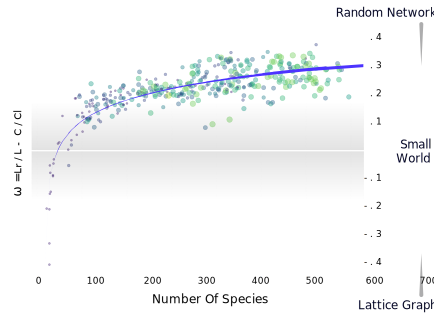
\includegraphics[width=\textwidth]{figures_c3/logpart.pdf}
        \caption{\textbf{A figure showing the small worldness for many Monte-Carlo selected MCM subsets}. The network structure of these is then assessed using the omega coefficient, with [-1,0,1] corresponding to the perfect lattice, small-world and random network structure. Here Node size and colour represents the number of reactions in the subset and the number of primary VOCs (blue=small, green=large).}
        \label{fig:smw}
\end{figure}



\subsection{Power Law and Scale-free graphs}
In real-world applications, it is common to have a hierarchical structure. These are often seen in the increase of citation counts in academic papers \citep{scalefreepapers}, email threads \citep{scalefreeemail} and the world wide web \citep{neoj4}. Unlike random or small-world graphs, scale-free graphs take a hub-and-spoke structure (\autoref{fig:gstructure}), which follows a power-law distribution - that is that scaling probability $p(x) \propto x^{-\alpha}$, where $\alpha$ is a constant and known as the scaling parameter.

\cite{scalefreebad} suggests that scale-free networks are rare, and often misdiagnosed with incorrect tests, or the misinterpretation of power-law features in a network. Similarly, \cite{plexp} suggests that even if the data distribution of a graph is well represented by the power-law distribution, in many cases a logarithmic or exponential distribution may have a better fit. 

\begin{figure}[H]
     \centering
         \includegraphics[width=.8\textwidth]{figures_c3/graphstyles.png}
        \caption{\textbf{The different network structures}. A visual depiction of the different graph structures. Source: \cite{neoj4}}
        \label{fig:gstructure}
\end{figure}

To assess the best distribution for describing the monte carlo subsets of the MCM I use the Kolomogorov-Smirnov statistic \citep{ks}. This calculates the maximum distance $D$ between the selected cumelative distribution function $S(x)$ (In our case the Logarithmic, Exponential and Power Law) of the data and the fitted model $P(x)$:

\begin{equation}
D = \smash{\displaystyle\max_{x \ge x_{min}}} |{S(x) - P(x)}|
\end{equation}

Using the MCM subsets from before \autoref{fig:ksd} shows that out of the three tested distributions, the MCM is best represented as a power-law distribution. Although this is not entirely within the chosen 5\% significance, it is highly indicative that some aspects of the network are scale-free.

\begin{figure}[H]
     \centering
         \includegraphics[width=\textwidth]{figures_c3/KSdistance.png}
        \caption{\textbf{Comparing the MCM subsets against a power law, logarithmic and exponential distribution.} The fit for different cumulative probability distributions of nodes in the MCM network is compared to determine the type of network hierarchy the chemistry follow. This is done by comparing the distance of the calculated distribution of data against a perfect one using the Kolomogorov-Smirnov test. The closer the two distributions are the better the fit. }
        \label{fig:ksd}
\end{figure}

\subsection{Describing the MCM network}
To conclude the MCM network exhibits both small world and scale-free (power-law) characteristics. This agrees with previous knowledge about the apparent network structure (branch and core - ref CH1/2). Here large primary emitted hydrocarbons produce branches of a hierarchical nature, as they are progressively broken down into smaller species. Since smaller species are then able to react with a much greater range of species, they then begin to form a tightly connected core, which exhibits many small-world features. This can be seen as the densely connected region within the graphs in CHAPTER !. 

Having classified the MCM network type, the next section will look at how MCM based simulation results can be converted into the graph structure for more in-depth analysis, \autoref{sec:metriccase}.


\section{Graph Construction methodology }\label{sec:chem}

Thus far we have only applied a qualitative analysis on the relationships between species in a mechanism. Although this can educate us about the chemistry within a specific system, often a quantitative value for the rate of reaction between different species is required when undergoing scientific evaluation or policy advice. To obtain such results a chemical mechanism is placed within an atmospheric model, initial concentrations are supplied and the chemistry is propagated forwards\footnote{Or backwards if the adjoint is used. (see section PAGERANK APPLICATIONS)} in time. Currently, there exist three main model diagnostics which we may use to analyse the importance or role of a species from a simulation (model) output. 


\subsubsection{Concentration time series}

The simplest of these methods look at the abundance of a  species at a specific point in the atmosphere - its concentration. As time moves forwards, chemicals within the atmosphere undergo a range of reactions which result in the making and breaking of bonds - thus the changing from one species to another. 

Using the species concentration as a metric, we can map how it changes over time, and how in changing the initial concentrations of a simulation can produce different results. This can be useful for looking at a range of possible scenarios and evaluating the potential outcome after a pre-determined amount of time. An example would be through the use of policy-based simulations to predict changes in ...

Using a simple example from a Methane only subset of the MCM (\autoref{fig:concentration}), it is possible to observe the inverse relationship between \ch{NO2} and \ch{NO} using only their concentration profiles. Here nitrogen monoxide reacts with a \ch{Ro2} species to produce an RO and nitrogen dioxide.
This then photolyses back to nitrogen oxide, releasing oxygen which may go on to form ozone (REF NOX CYCLE IN INTRO). The latter part of this reaction is dependant on photons and therefore can only occur during daytime (mostly).
 
\begin{figure}[H]
     \centering
         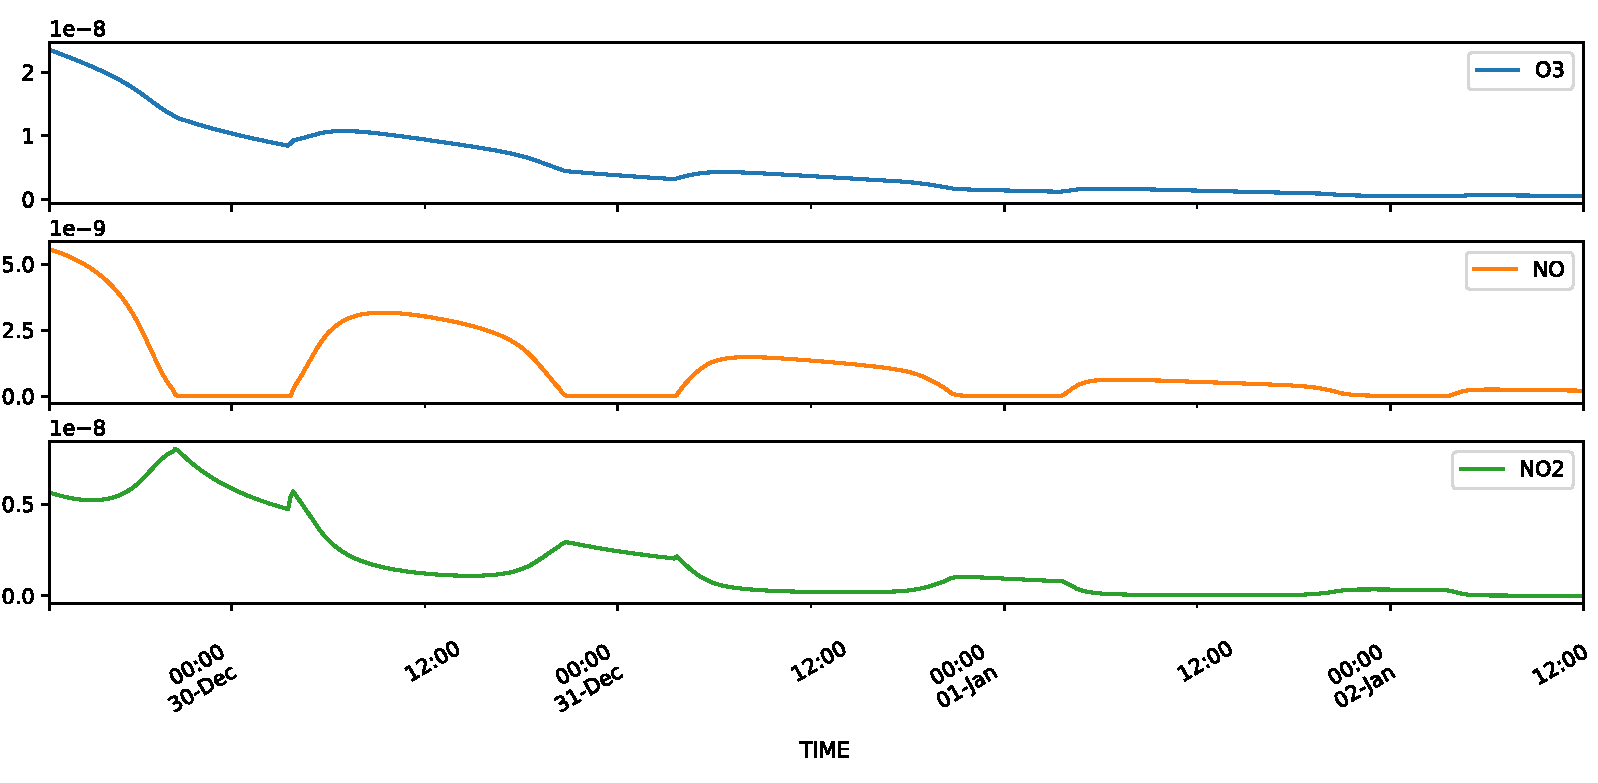
\includegraphics[width=.85\textwidth]{figures/ch2concentration.pdf}\\
         \ce{NO <-->[RO2][$hv$] NO2}.
        \caption{\textbf{A concentration time series from a simple methane-only simulation.} This is the simplest method for identifying changes in species within a model simulation. This multi-plot shows the changes in concentration profiles for all initialised species (NOx:10ppb; \ce{CH4}:20ppb; \ce{O3}:30ppb) following an initial 3 day spin-up to steady state. }
        \label{fig:concentration}
\end{figure}

\subsubsection{Rate of Production and Loss}

Analysing the concentration-time profiles allows the comparison of how a series of scenarios or runs change concerning their initial conditions and simulation length. Although these can tell us how, and how much, each species changes over time it does not rank or quantifies the specific reactions to which this may be attributed. Rate of Production Analysis (ROPA)\footnote{and loss} provides a method for establishing the total contribution from each reaction by calculating the change of concentration (concerning time) for the produced species - the instantaneous reaction Flux.

\begin{eqnarray}
  r_1 = \eta A + \omega B \overset{\kappa_1}{\xrightarrow{\hspace*{7mm}}} C & & \text{ Reaction 1}\\[15pt]
  f(C) = \dfrac{\delta C}{\delta t} =  [A][B]\  \eta \omega \times \kappa_1                      & & \text{ Instantanious Flux }(\Gamma) \label{eqn:ode}
\end{eqnarray}

Here A, B and C are example species; [A],[B] and [C] are species concentrations; $\eta$ and $\omega$ are rate coefficients and $\kappa$ is the rate of the reaction.  

Using a sample simulation representative of the conditions within Beijing (an urban environment), we explore the reactions contributing to the production and loss of \ch{CH3CO3},
\autoref{fig:ropa_day} at noon. The main reason for this specific example is that it can demonstrate how isolating a specific cause for the change within a species concentration may prove difficult in the context of atmospheric chemistry. Here we have many similarly weighted production and loss reaction, including that of peroxyacetyl nitrate (PAN) and nitrogen dioxide: 
\ce{CH3CO3 + NO2 <--> CH3C(O)ONO2} (PAN). The reversible nature, coupled with its near-identical production and loss fluxes produce a very small net change within our species of interest (\ch{CH3CO3}). Although this may be seen by calculating the cumulative flux between individual species, it is evident that simply looking at the concentrations or highest-ranking reaction fluxes may not be the best method of determining influence. To account for this we can look at how a change in one species can affect another using the Jacobian method.


\begin{figure}[H]
     \centering
         \includegraphics[width=\textwidth]{figures/ROPA_CH3CO3.pdf}
        \caption{\textbf{Rate of production and loss analysis plot for \ch{ch3co3} exhibiting a net loss (daytime).} An example ROPA plot from a simulation representing the chemistry within Beijing. This is used to identify the usefulness and weaknesses of using such a method.}
        \label{fig:ropa_day}
\end{figure}
\newpage



\subsubsection{The Jacobian}
"The Jacobian [matrix] generalises the notion of gradient to describe the sensitivity to a vector" - \cite{jacob}. That this means is that in taking the partial derivatives of each reaction flux (e.g. from \autoref{eqn:ode}), we can construct a representation of the influence each species has on itself - for example, the influence of species A on C and B on C (\autoref{eqn:A}-\ref{eqn:B}). 
\begin{eqnarray}
   \dfrac{\partial \ }{\partial A}\cdot \dfrac{\partial C_{r_1}}{\partial t} = \eta \omega B \kappa_1 & & \Gamma \text{ influence from A }\label{eqn:A}%\\[15pt]
\end{eqnarray}
    
\begin{eqnarray} 
   \dfrac{\partial \ }{\partial B}\cdot \dfrac{\partial C_{r_1}}{\partial t} = \eta \omega A \kappa_1 & &  \Gamma \text{ influence from B }\label{eqn:B}%\\[15pt]
\end{eqnarray}
      
These partial equations can then be aggregated for all reactions that contain the two species - taking the effect of species B on species C, for example, produces \autoref{eqn:Bsum}. Using these aggregate sums it is now possible to construct a pairwise relational matrix describing the influence each species has on every other species- \autoref{eqn:jacadj}. This is known as the jacobian matrix and is what is used to propagate the chemistry within a simulation forwards in time. 
 
               
\begin{eqnarray}
   \mathbf{J}_{C,B} = \dfrac{\partial f(C) }{\partial B} =
\dfrac{\partial \ }{\partial B} \cdot \left( \dfrac{\partial \Sigma_{r_1}}{\partial t} + \dfrac{\partial \Sigma_{r_2}}{\partial t} + \cdots +\dfrac{\partial \Sigma_{r_n}}{\partial t} \right)
\label{eqn:Bsum}
\end{eqnarray}\\

\begin{eqnarray}
 \mathbf{J}_{i,j} =
 \begin{bmatrix}
   \dfrac{\partial f_1}{\partial v_1} &
     \dfrac{\partial f_1}{\partial v_2} &
     \cdots &
     \dfrac{\partial f_1}{\partial v_n} \\[13pt]
   \dfrac{\partial f_2}{\partial v_1} &
     \dfrac{\partial f_2}{\partial v_2} &
       \cdots &
     \dfrac{\partial f_2}{\partial v_n} \\[13pt]
       \vdots &
     \vdots & \ddots
        &
     \vdots\\[13pt]
   \dfrac{\partial f_n}{\partial v_1} &
     \dfrac{\partial f_n}{\partial v_2} &
       \cdots &
     \dfrac{\partial f_n}{\partial v_n}
 \end{bmatrix}_{i,j=1}^{n,n}
 \label{eqn:jacadj}
\end{eqnarray}



\subsection{Graph construction methodology for simulated data}\label{sec:graphconstruction}

Having covered the general definition of a Jacobian matrix and how it is constructed, we can now apply it to the context of mechanism analysis and comprehension. The first analogy that needs to be made is that for the flux, we have a the first differential of a specific reaction in time. If we consider the change in a species concentration as a `displacement', we can think of the flux as its `velocity'.
Similarly, the Jacobian provides us with a description of how the individual flux of a species changes concerning the concentration (or displacement) or another species (the second-order partial differential). This is analogous to the acceleration of the object or particle we first displaced. In using the jacobian, we have constructed a relational matrix which outlines the effect a 1\% change of a species has on all other species - a concept which is the foundation of the connectivity method (a mechanism reduction technique where all but essential and important species are removed), \citep{connectivity}.

Since the format of a jacobian is already in the form of a relational matrix, it can easily be converted to a weighted adjacency matrix, and then directly into the graph format. Since it only considers the aggregated influence between species, much of the work that would otherwise be needed to convert a mechanism into a graph format has already been done. To make use of the Jacobian matrix, several extraction algorithms were written for an updated version of the Dynamically Simple Model of Atmospheric Chemical Complexity (DSMACC) [DANDSMACC,DSMACC ref], as discussed in INTRODUCTION. Here we edit the kinetic pre-processor output, \citep{kpp} to release the values of the Jacobian Matrix and return them at each model timestep for analysis. The process for how this is done is described in \autoref{sec:jacpractical}.



\subsubsection*{ A note on using the Flux instead of the Jacobian }
Depending on the model setup or the users' capabilities, extraction of the jacobian matrix for each timestep may not be possible. In many cases, the reaction rates and concentration may still be available, allowing for the calculation of reaction fluxes throughout the simulation. If this is the case the total flux can be calculated using the method described in  \autoref{eqn:ode}. From this, an edge-weighted by a reaction flux can be created from every reactant to each product. This generates a multi-graph\footnote{A graph with multiple edges between nodes} which may be simplified by taking the net flux value for all edges between two nodes. 

However, the potential for human/coding error, additional simplification and a non-explicit definition of the contribution of each species make the use of a Jacobian much more efficient in network generation from a chemical mechanism. 


\subsection{A practical Example using the MCM}\label{sec:jacpractical}

Taking a single equation from the MCM we may calculate the jacobian relationships between species and convert them into a graph. A randomly chosen ethane reaction (\autoref{eqn:line}) from a simple mechanism was chosen. It must be noted that in general it is unusual in the MCM that alkyl radicals react rapidly and extremely well with \ce{O2} to from stabilised peroxy radicals, \citep{mcmorigin}. In general, the reaction would consist of the following two steps:
 \ce{C2H6 + OH ->[\kappa_1] C2H5. + H2O}
and \ce{C2H5. + O2 -> [\kappa_2] CH2H5O2}.

\begin{equation}
\label{eqn:line}
\ce{C2H6} + \ce{OH} \overset{\kappa_3}{\xrightarrow{\hspace*{7mm}}} \ce{C2H5O2}
\end{equation}

For simplicity in this example, this will be the only equation for our mechanism. The resultant Flux \autoref{eqn:exflux} and resultant Jacobian \autoref{eqn:exjac} may be calculated.

\begin{equation}\label{eqn:exflux}
   \Gamma = [\ce{C2H6}][\ce{OH}]\kappa_1 \\[15pt]
\end{equation}

   \begin{eqnarray}
    \mathbf{J}_{i,j} =
 \begin{bmatrix}
   \dfrac{\partial f_{[\ce{C2H6}]}}{\partial t \ \partial {[\ce{C2H6}]}} &
     \dfrac{\partial f_{[\ce{C2H6}]}}{\partial {[\ce{OH}]}} &
     \dfrac{\partial f_{[\ce{C2H6}]}}{ t \partial {[\ce{C2H5O2}]}} \\[20pt]
   \dfrac{\partial f_{[\ce{OH}]}}{\partial t \ \partial {[\ce{C2H6}]}} &
     \dfrac{\partial f_{[\ce{OH}]}}{\partial t \ \partial {[\ce{OH}]}} &
   \dfrac{\partial f_{[\ce{OH}]}}{\partial t \ \partial {[\ce{C2H5O2}]}} \\[20pt]
   \dfrac{\partial f_{[\ce{C2H5O2}]}}{\partial t \ \partial {[\ce{C2H6}]}} &
     \dfrac{\partial f_{[\ce{C2H5O2}]}}{\partial t \ \partial {[\ce{OH}]}} &
     \dfrac{\partial f_{[\ce{C2H5O2}]}}{\partial t \ \partial {[\ce{C2H5O2}]}}
 \end{bmatrix}_{i,j=1}^{3,3}
 \label{eqn:exjac}
\end{eqnarray}\\


Since not all species react with all other species, we can remove reactions that do not exist. This forms a `sparse' jacobian. Substituting numbers from a subset mechanisms containing the methane and ethane precursors, we get \autoref{eqn:exjacsp}.


   \begin{eqnarray}
    \mathbf{J}_{i,j} =
 \begin{bmatrix}
   \dfrac{\partial f_{[\ce{C2H6}]}}{\partial t \ \partial {[\ce{C2H6}]}} &
     - 2\times 10^{-7} &
     2\times 10^{-7} \\[20pt]
   -0.1 &
     \dfrac{\partial f_{[\ce{OH}]}}{\partial t \ \partial {[\ce{OH}]}} &
  0.1 \\[20pt]
   \  &
    \  &
     \dfrac{\partial f_{[\ce{C2H5O2}]}}{\partial t \ \partial {[\ce{C2H5O2}]}}
 \end{bmatrix}_{i,j=1}^{3,3}
 \label{eqn:exjacsp}
\end{eqnarray}\\


This allows us to see two things. Firstly that with the absence of external intervention (e.g. emissions) the overall change of concentration is a conserved property. Secondly ...\\

Representing these relationships as a simple `ball and link' style graph gives us \autoref{fig:jacgraph}.

 \begin{figure}[H]
 \begin{center}
 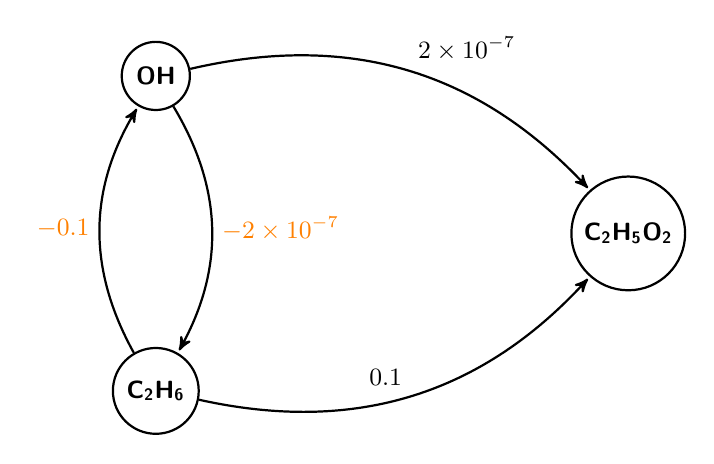
\begin{tikzpicture}[->,>=stealth',shorten >=1pt,auto,node distance=7cm,
                    thick,main node/.style={circle,draw,font=\sffamily\small\bfseries}]

  \node[main node] (1) at (1,4){\ce{OH}};
  \node[main node] (2) at (1,0) {\ce{C2H6}};
  \node[main node] (3) at (7,2) {\ce{C2H5O2}};

  \path[every node/.style={font=\sffamily\small}]
    (1) edge [bend left] node {$2 \times 10^{-7}$} (3)
     (2) edge [bend right] node {$0.1$} (3);

     \path[every node/.style={font=\sffamily\small,color=orange}]
     (1) edge [bend left] node {$-2\times 10^{-7}$} (2)
     (2) edge [bend left] node {$-0.1$} (1);

        %edge [loop left] node {0.4} (2)
        %edge [bend right] node[left] {0.1} (3);
    %(3) edge node [right] {0.8} (2);
\end{tikzpicture}

 \end{center}

\caption{ A graphical representation of \autoref{eqn:exjacsp} derrived from the \autoref{eqn:line}}\label{fig:jacgraph}
 \end{figure}

\paragraph{Converting the Jacobian into an adjacency matrix}
Adjacency matrixes are a set of matrix representations which can be used in the construction of a graph. The relational data of the Jacobian matrix \autoref{eqn:exjacsp} inherently holds such property and can be directly translated to produce a graph, \autoref{fig:jacgraph}. However, we notice that some edge weights are negative, which although providing information about the chemical system provides no physical meaning in the graph structure.

It is for this reason that we can reverse the direction for all negative links to produce \autoref{fig:jacgraphnonneg}.

\begin{figure}[H]
\begin{center}
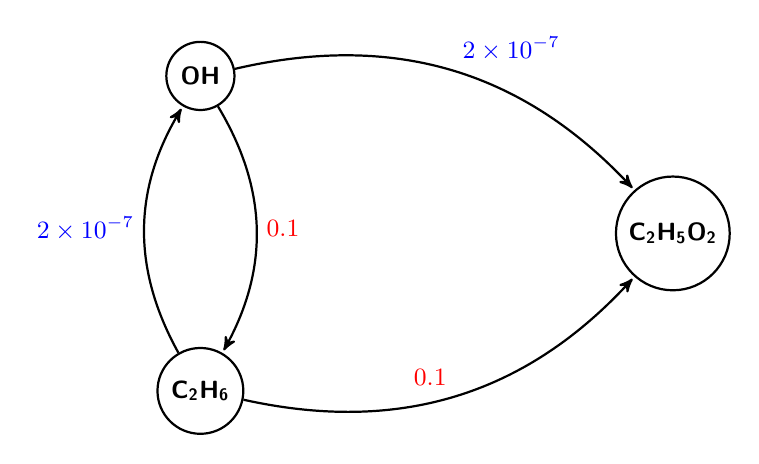
\begin{tikzpicture}[->,>=stealth',shorten >=1pt,auto,node distance=7cm,
                   thick,main node/.style={circle,draw,font=\sffamily\small\bfseries}]

 \node[main node] (1) at (1,4){\ce{OH}};
 \node[main node] (2) at (1,0) {\ce{C2H6}};
 \node[main node] (3) at (7,2) {\ce{C2H5O2}};

 \path[every node/.style={font=\sffamily\small,color=blue}]
   (1) edge [bend left] node {$2 \times 10^{-7}$} (3)
   (2) edge [bend left ] node {$2\times 10^{-7}$} (1);
   \path[every node/.style={font=\sffamily\small,color=red}]
   (1) edge [bend left] node {$0.1$} (2)
  (2) edge [bend right] node {$0.1$} (3);
\end{tikzpicture}

\end{center}

\caption{ Reversing the directions on negatively weighted edges from \autoref{fig:jacgraph}}\label{fig:jacgraphnonneg}
\end{figure}


For most graph algorithms this should be sufficient and is generally all that is needed. In some cases, it may, however, be noted that the graph may further be simplified to produce \autoref{fig:jacgraphsim}. Although this is more practical, eigenvector metrics such as PageRank will automatically transfer the `flow' of information down the system producing much the same overall result.

\begin{figure}[H]
\begin{center}
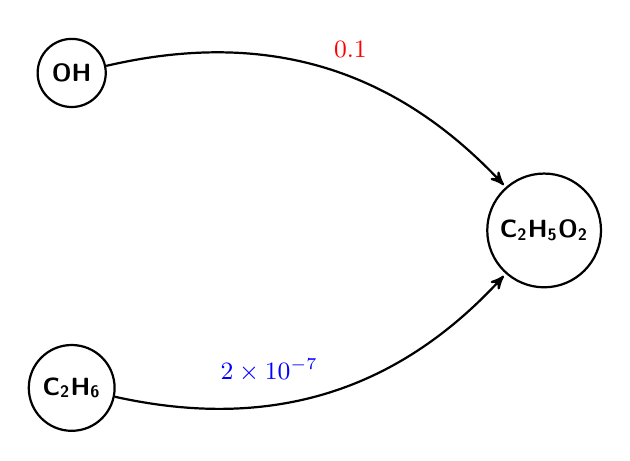
\begin{tikzpicture}[->,>=stealth',shorten >=1pt,auto,node distance=7cm,
                   thick,main node/.style={circle,draw,font=\sffamily\small\bfseries}]

 \node[main node] (1) at (1,4){\ce{OH}};
 \node[main node] (2) at (1,0) {\ce{C2H6}};
 \node[main node] (3) at (7,2) {\ce{C2H5O2}};

 \path[every node/.style={font=\sffamily\small,color=blue}]
   (2) edge [bend right] node {$2 \times 10^{-7}$} (3);
   \path[every node/.style={font=\sffamily\small,color=red}]
  (1) edge [bend left] node {$0.1$} (3);
\end{tikzpicture}

\end{center}

\caption{ Simplifying \autoref{fig:jacgraphnonneg}}
\label{fig:jacgraphsim}
\end{figure}



\section{Case study Example}\label{sec:metriccase}
In this section the centrality metrics discussed in \autoref{sec:graphcentrality} are applied to a range of senarios. These range from polluted urban environments such as London [REF] and Beijing [REF], to marine and terrestial forrest- Cape Verde REF and Borneo REF. We determine the main drivers for the chemistry and compare the species which are important across each simulation.  

\subsection{Establishing Initial Conditions from observational data}
Within experimental data assimulation it is not uncommon to face problems which resut in unreliable or missing data. These can range from anything as little as measuring below the instrument sensitivity to powercuts and equiptment damage/theft from the local wildlife. This can result in problems when analysing the results and combining them to create a simulation of the chemistry for that environment. 

To overcome this, traditionally a combination of data filtration, smoothing and interpolation is required. Although it is possible to fit a diurnal profile, through itereative methods of comparison, and cubic splines, a much simpler way would be to use an Multi Layer Perceptron Regressor model (MLPRegressor) as provided by sklearn, \citep{sklearn}. This is described below.

\subsubsection{The origin of Artificial Neural Networks}
The concept of a neural network originated witin the field of neuroscience. In in bilogical neurons, signals are sent through the use of electrical impulses using their synapses. When a sufficient number of signals are recieved within a short timeframe, a neurone will respond, often firing a range of its own signals. Using this as a foundation,\cite{pitts} presented a computational model of the biological neuron - the artifical neuron. This has a series of binary inputs, and produces a single binary output. This idea was later imporoved with the invention of the perceptron - a linear classifier which classifies categories by separating them with a straight line. Invented by \cite{perceptron}, this was popularised as a device representative of a modern day shallow neural network - \citep{perceptronmanual}, \autoref{fig:perceptron}. Unlike the artificial neuron however, the perceptron is able to take non-binary (numerical) inputs of an associated weight which allows for the computation of simple linear binary classification. Much like Logistic regression, the preceptron produces a positive or negative classification based on a certain threshold\footnote{It is worth noting that while a Logistic Regression classifier can output a class probability, the use of a hard threshold means that this is not done within the preceptron algorithm \citep{handsonml}}. 


\begin{figure}[H]
     \centering
         \includegraphics[width=.45\textwidth]{figures_c3/mlpregressor/Mark_I_perceptron.jpg}
        \caption{\textbf{The Mark 1 perceptron} Both software and hardware are different manifestations of a flow chart. The perceptron hardware accomplished what is now done using software. Source: \cite{perceptronimage}}
        \label{fig:perceptron}
\end{figure}

\subsubsection{The Multi Layer Perceptron}
Limitations of ther perceptron include the classifiction of complex patterns such as the XOR problem (where a category appears between two other categories e.g. {1|0|1} - this cannot be classified by a single linear split). In taking inspiration from nature, \autoref{fig:layercortex}, it is possible to overcome this with the use of multiple layers. This creates an a deep ($>2$ two hidden (non-input) layers of perceptrons\footnote{These are sometimes refered as Linear Threshold Units.}) artificial neural network (ANN) 

The multi layer perceptron (MLP) model now represents a simple feed-forwards network, much like a decision tree. However unlike a decision tree, the MLP ANN is able to describe the probability a branch is taken using non-linear activation (threshold) functions. These are discussed in detail as part of \autoref{sec:ae}. The weighting thresholds for each neuron are then calculated by backwards propagation of results through the network until a suitably good result is produced. 

\begin{quote}
\textit{
\textbf{Example analogy:} Back propagation can be likened to the iterative calibration of scientific instrumentation. In the field of atmopsheric chemistry laser induced flourecence is used to calculate species concentrations and reaction rates within the troposphere, \citep{lif1,lif2}. Here the frequency of a laser can be adjusted in contrast with a known target (e.g. an amount of \ce{SO2}) to produce a responce curve showing where the maximum resonance occurs.\\
Similarly a neural network can be `trained' (calibrated). 
This is done through the use of a `training dataset' - a set of input-output pairings which represent a random selectaion of 2/3rds of the total dataset. Next the neurons within each layer (similar to the potentiometer dials on an instrument) are adjusted in sequence through the layers to match the known result (a standard of known concentration) to the input values provided. This process is repeated until for a number of iterations, or until a sufficently `good' prediction is attained for the entire training dataset (early termination). The power of ANNs comes from the ability to adjust neuron thresholds whilst moving both forwards and backwards through the network (Note: predictions of a MLP are still only passed forwards). Finally model perfomance is evaluated against the remaining 1/3rd of the total dataset.
}
\end{quote}


\begin{figure}[H]
     \centering
         \includegraphics[width=.85\textwidth]{figures_c3/mlpregressor/Cajal_cortex_drawings.png}
        \caption{\textbf{The Human Cortex - A biological neural network.}. A vertical cross section of the human cortex between an adult (top) and 1.5 month old infant (bottom) showing a layer like structure with a change in depth (left to right). Source: \cite{layercortex}}
        \label{fig:layercortex}
\end{figure}

\subsubsection{Applying the MLPRegressor to Observational data}
In the application of any type of machine aided algorithms it is important to evaluate the results provided. In this section the results of 12 years of data collected as part of the [CAPE VERDE CAMPAIGN] are shown (these contain measurements spanning the entirety of 12 years, which produce the clearest tests for the algorithm). A MLPRegressor of 10 hidden layers, and a hyperbolic tan (tanh) activation function is used \autoref{sec:appendix:tanh}. Additionally the limited-memory Broyden–Fletcher–Goldfarb–Shanno (l-BFGS) solver (a quasi-newton method which minimises the inverse of the Hessian matrix\footnote{ The hessian is square matrix of second-order partial derivatives of a scalar-valued function/field describing the local curvature of a function (of many variables).} to steer through space and obtain a solution) and an adaptive learning rate\footnote{Each time the model improvement fails to decrease the learning loss, the learning rate is reduced by 1/5. This means smaller jumps are made towards the curve peak. } is used. 

Input of the regressor is in the from of a month and a hour, to represent each measurement. This allows it to find not only daily trends, but also seasonal trends within the data. Once trained the regressor is then used to predict a diurnal profile for each month based on the observational data provided. For simplicity $\log_{10}$ values of the concentrations obtained have been used. To validate the results, the predicted MLPRegressor line is compared to a transparent scatterplot for all the results. In addition to this a boxplot showing the IQR, median and mean (green line) plotted alongside to evaluate the predictor output. 

In providing the MLPRegressor with both month and hour inputs, the data is not only fitted hourly (a diurnal avarage), but also across the seasonal/monthly cycles. This accounts for the variation between years and datasets. Since $\log_{10}$ values of the concentrations are used, species such as ozone (\autoref{fig:mlpo3}) which for the Cape Verde dataset (clean air) do not change more than one order of magnitude, the effects of neigbouring months, which shift the diurnal away from the mean (the green line on the boxplot), can be seen. However since this is overall a small change, and the diurnals lie within the inter quartile range, they still provide an adequate approximation. NO (\autoref{fig:mlpno}) on the other hand has a concentration change of several orders of magnitude. Here a distinct daytime peak is seen and is centred around a sesonally consistent mean value of the data. Here the multi-magnitude change in concentration also provides an effective silhouette of the data to which we may compare the fitted line. 
Finally the plots of \ce{NO2} and iso-Pentane (\autoref{fig:mlpno2}-\ref{fig:mlpisopentane}) vary both in diurnal magnitude and seasonally. Within these plots, changes in the data in the january and december months produce deceptively misleading results. Here although the diurnals are not symmetrix, they fit well within the median,mean and interquartile range values, as well as the general data silhouette behind them. This siggests that it is a property of the data that we are fitting, and not that the regressor is producing incorrect results. It is however noted that for a more accurate seasonal prediction, periodic boundary conditions should be employed in the training dataset, where an additional two months are added before January and after December. As only a single value estimate from the summer region will be taken, this does not affect the result accuarcy. 

\begin{figure}[H]
     \centering
         \includegraphics[width=.90\textheight,angle =90,trim={8cm 0 0 0}]{figures_c3/mlpregressor/CVNOX_CapeVerde/O3.pdf}
        \caption{\textbf{Cape Verde MLP predicted and observational data of Ozone.} Each segment represents data from a different month. Within each month segment exists 24 hour segments to create a diurnal. Observational concentrations are plotted in the form of a translucent scatterplot and summarised using the boxplot on the right of the month segment. MLP predicted results are shown using the solid lines. Concentration in mixing ratio.}
        \label{fig:mlpo3}
\end{figure}

\begin{figure}[H]
     \centering
         \includegraphics[width=.90\textheight,angle =90,trim={8cm 0 0 0}]{figures_c3/mlpregressor/CVNOX_CapeVerde/NO.pdf}
        \caption{\textbf{Cape Verde MLP predicted and observational data of NO.} Each segment represents data from a different month. Within each month segment exists 24 hour segments to create a diurnal. Observational concentrations are plotted in the form of a translucent scatterplot and summarised using the boxplot on the right of the month segment. MLP predicted results are shown using the solid lines. Concentration in mixing ratio.}
        \label{fig:mlpno}
\end{figure}

\begin{figure}[H]
     \centering
         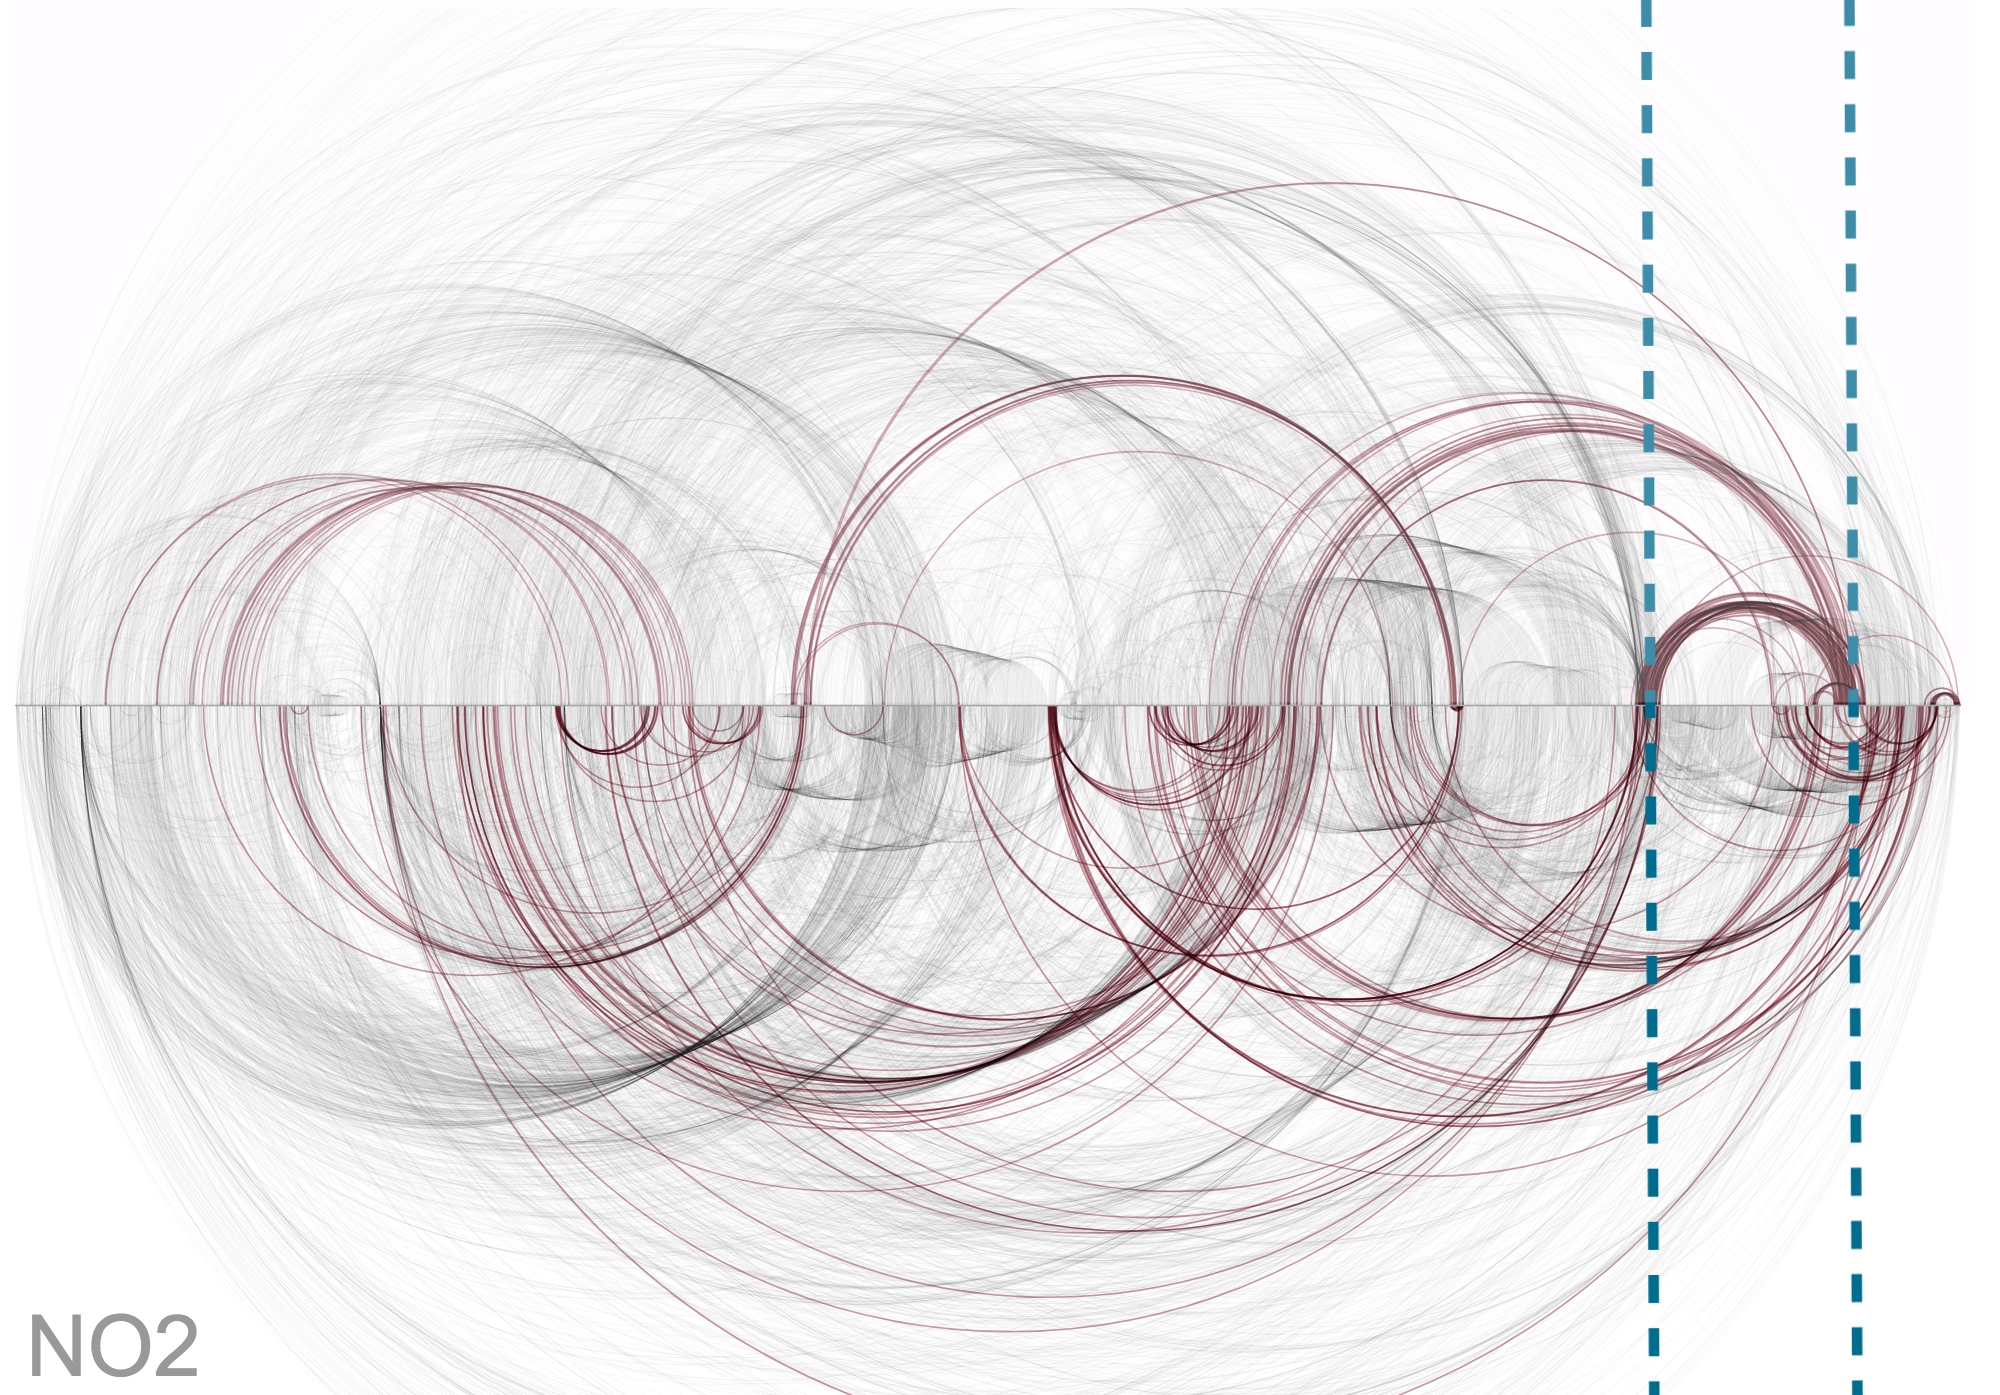
\includegraphics[width=.90\textheight,angle =90,trim={8cm 0 0 0}]{figures_c3/mlpregressor/CVNOX_CapeVerde/NO2.pdf}
        \caption{\textbf{Cape Verde MLP predicted and observational data of \ch{no2}.} Each segment represents data from a different month. Within each month segment exists 24 hour segments to create a diurnal. Observational concentrations are plotted in the form of a translucent scatterplot and summarised using the boxplot on the right of the month segment. MLP predicted results are shown using the solid lines. Concentration in mixing ratio.}
        \label{fig:mlpno2}
\end{figure}

\begin{figure}[H]
     \centering
         \includegraphics[width=.90\textheight,angle =90,trim={8cm 0 0 0}]{figures_c3/mlpregressor/CVNOX_CapeVerde/ISO_PENTANE.pdf}
        \caption{\textbf{Cape Verde MLP predicted and observational data of iso-Pentane.} Each segment represents data from a different month. Within each month segment exists 24 hour segments to create a diurnal. Observational concentrations are plotted in the form of a translucent scatterplot and summarised using the boxplot on the right of the month segment. MLP predicted results are shown using the solid lines. Concentration in mixing ratio. }
        \label{fig:mlpisopentane}
\end{figure}


\subsubsection{Model Initialisation Procedure}
The aim is to genearate a set of intiation concentrations which are representative of the different types of chemistry between environments. In this section we are not interested in the exact concentration modelling for specific times or senarios. Instead we seek to generate representative of the processed chemistry under a range of conditions. 

To do this species concentrations are extracted from a MLP regressior trained on observational data for each senario. Each concentration is that of 12:00 local time from the generated diurnal from summer obsrevations at each location. This produces a montly error of $\pm 2 months$ from June. As both nitrogen oxide and dioxide are supplied the total NO$_x$ for each simulation are \emph{not} constrained. The initial conditions are shown in \autoref{tab:icsmetric}.

In general observational measurements are not able to detect all the species presented within the MCM. This means that in order to be able to compare model senarios, the chemistry must first be spun up. In propatating the chemistry forwards in time, primary emitted and measued species are broken up forming the intermediate species which exist within a mechanism. In order to reach steady state, the model is initated at noon and the observational concentrations are rest every 24 hours. For each diurnal the fractional difference between the concentrations at each day are compared. If the difference between these is less than 0.001, the model is left to run unonstrained for 5 days (right of the dashed line in \multiref{fig:ccape}{fig:cbeijing}). Model results are then taken after 3 days of unconstrained runs. The reason for this is that the total RO$_2$ concentration takes longer to stabilise in the polluted environments (London and Beijing). This falls into a periodic cycle beginning noon on the third day, and can provide a representation of the processed chemistry within each environment. 

\textit{NOTE: It should be noted that some of the concentration plots may appear to lose their diurnal dependability. This may be attributed to the changing order of magnitude of the concentrations, and that the species are still responding as expected. }

\subsubsection{Extracting the required results}
Model diagnostics such as concentration and the net flux passing through a species may be extracted directly from the DSMACC box model. These provide the baseline comparison and can be directly compared to the graph metrics. Species concentration tells us the abundance of different species, and the net-flux tells us how fast this is changing with respect to time. 

As some species may have a fast inwards and outwards flux (low net-flux), the aboslute flux is also included. Finally the sensetivity of each species with respect to other species is also extracted (the jacobian matrix). This serves to not only generate the graph used to represent the chemistry, (\autoref{sec:graphconstruction}), but also to identify the overall influence a species has on others in the network. This can be calculated by taking the net sum of the influence a species has on every other from the Jacobian. This is analogous to calculating the outdegree of a node in the jacobian network. 
\newpage
 
\begin{table}[H]
\centering
\small


\begin{table}[H]
\centering
\small

%%%%%%%
\begin{tabular}{p{0.2\textwidth}p{0.16\textwidth}p{0.16\textwidth}p{0.16\textwidth}p{0.16\textwidth}}
\toprule
Species & Beijing(APHH) & Borneo(OP3) &  London(ClearFlo) &  CapeVerde \\
\midrule
\ce{LAT}       & 39.9 &              0.96 &            51.0&       16.5 \\
\ce{LON}       &  116.3 &              114.5 &            0.00 &       23.4 \\
\midrule
CO & 3.829e-06 & 3.321e-07& 7.780e-09 & 0.0*\\
\ce{O3}        &  6.883e-08 &              8.939e-09 &            3.819e-08 &       2.629e-11* \\
\ce{NO}        &  1.660e-09 &              2.668e-14* &            2.350e-09 &       2.358e-12 \\
\ce{NO2}       &  1.226e-08 &              1.081e-13* &            7.445e-09 &       8.447e-12 \\
\ce{HCHO}      &  4.472e-09 &                        &            1.119e-08 &                 \\
\ce{C2H6}      &  3.163e-09 &              7.315e-10 &            2.133e-09 &       4.539e-10 \\
\ce{C2H4}      &  1.004e-09 &              1.152e-10 &            4.893e-10 &       2.481e-11 \\
\ce{C3H8}      &  3.019e-09 &              1.924e-10 &            1.128e-09 &       1.728e-11 \\
\ce{C3H6}      &  1.335e-10 &              1.333e-11 &            1.784e-10 &       9.343e-12 \\
\ce{IC4H10}    &  6.412e-10 &              8.742e-11 &            5.142e-10 &       2.486e-12 \\
\ce{NC4H10}    &  1.593e-09 &              5.698e-11 &            1.058e-09 &       4.481e-12 \\
\ce{C2H2}      &  1.058e-09 &              1.825e-10 &            3.018e-10 &       1.848e-11 \\
{TBUT2ENE}  &  4.198e-11 &                        &            1.815e-11 &                 \\
{CBUT2ENE}  &  4.454e-11 &                        &            1.305e-11 &                 \\
\ce{IC5H12}    &  1.047e-09 &              2.883e-11 &            7.424e-10 &       3.470e-12 \\
\ce{NC5H12}    &  4.650e-10 &              2.090e-11 &            2.792e-10 &       2.513e-12 \\
{TPENT2ENE} &  3.939e-11 &                        &                      &                 \\
{CPENT2ENE} &  3.982e-11 &                        &                      &                 \\
\ce{NC6H14}    &  2.057e-10 &              6.437e-12 &            6.357e-11 &                 \\
\ce{C5H8}      &  7.134e-10 &              1.957e-09 &            1.640e-10 &                 \\
\ce{NC7H16}    &  7.905e-11 &                        &            5.222e-11 &                 \\
\ce{BENZENE}   &  4.045e-10 &                        &            1.137e-10 &       7.682e-12 \\
\ce{NC8H18}    &  3.091e-11 &                        &            1.442e-11 &                 \\
\ce{TOLUENE}   &  6.767e-10 &                        &            3.205e-10 &       3.121e-12 \\
\ce{EBENZ}     &  3.115e-10 &                        &            6.017e-11 &                 \\
\ce{OXYL}      &  1.677e-10 &                        &            5.049e-11 &                 \\
\ce{CH3CHO}    &  4.783e-10 &                        &            4.095e-09 &                 \\
\ce{C2H5OH}    &  4.655e-09 &                        &            3.125e-09 &                 \\
\ce{CH3COCH3}  &  3.328e-09 &                        &            2.924e-09 &                 \\
\ce{NC9H20}    &  1.336e-11 &                        &            7.922e-11 &                 \\
\ce{NC10H22}   &  1.062e-12 &                        &            1.602e-10 &                 \\
$\alpha$-\ce{PINENE}\footnotemark
   &  7.341e-11 &     15e-11                   &            1.105e-10 &                 \\
\ce{LIMONENE}  &  5.836e-11 &              1.351e-10 &            3.566e-11 &                 \\
\ce{PXYL+MXYL}\footnotemark
 &  4.943e-10 &                        &                      &                 \\
\ce{IPBENZ}    &  4.567e-10 &                        &                      &                 \\
\ce{PBENZ}     &  3.996e-10 &                        &                      &                 \\
\ce{HONO}      &  6.479e-10 &                        &            4.109e-10 &                 \\
\ce{MACR}      &            &              6.948e-11 &            1.862e-11 &                 \\

%%%%%%%%%%%%%%%
\bottomrule
\end{tabular}
\end{table}


\begin{table}[H]
\centering
\small
\begin{tabular}{p{0.2\textwidth}p{0.16\textwidth}p{0.16\textwidth}p{0.16\textwidth}p{0.16\textwidth}}
\toprule
Species & Beijing(APHH) & Borneo(OP3) &  London(ClearFlo) &  CapeVerde \\
\midrule

%%%%%%%%%%%%%%

{PENT1ENE}  &            &                        &            2.383e-11 &                 \\
\ce{MVK}       &            &                        &            2.091e-11 &                 \\
\ce{NPROPOL}   &            &                        &            2.883e-10 &                 \\
\ce{NBUTOL}    &            &                        &            4.535e-10 &                 \\
\ce{STYRENE}   &            &                        &            2.241e-11 &                 \\
\ce{MEK}       &            &                        &            5.494e-11 &                 \\
\ce{C3H7CHO}   &            &                        &            9.534e-12 &                 \\
\ce{C4H9CHO}   &            &                        &            1.865e-11 &                 \\
\ce{C5H11CHO}  &            &                        &            1.201e-11 &                 \\
\ce{CYHEXONE}  &            &                        &            9.790e-12 &                 \\
\ce{BENZAL}    &            &                        &            1.510e-11 &                 \\
\ce{PAN}       &            &                        &            1.791e-10 &                 \\
\bottomrule
\end{tabular}


\caption{(2-page split) The initial conditions created from the MLPRegressor prediction of observational data. Although not specified the concentration for methane is set by the model at 1770ppb, the temperature is 298K, and water vapour is at 2\%. \textbf{* Starred values are of the wrong units and should be multiplied by 1000. As there was no time to rerun these, their results have been omitted from this chapter.}}
\label{tab:icsmetric}
\end{table}

\footnotetext{This is written as ?-pinene in the merged CEDA dataset for the Borneo OP3 campaign. This is due to character conversion errors.}
\footnotetext{The concentration for these is split evenly between both species}

\caption{The initial conditions created from the MLPRegressor prediction of observational data. Although not specified the concentration for methane is set by the model at 1770ppb.}
\label{tab:icsmetric}
\end{table}

\footnotetext{This is written as ?-pinene in the merged CEDA dataset for the Borneo OP3 campaign. This is due to character conversion errors.}
\footnotetext{The concentration for these is split evenly between both species}
\newpage


\begin{figure}[H]
    \centering
\includegraphics[width=.9\textwidth]{figures_c3/mlpregressor/conc_cape.pdf}
\caption{\textbf{The concentration profile for CapeVerde.}This shows a the change in concentration over time for HO$_x$,NO$_x$,Ozone and RO$_2$ species for a simulation run generated by the mlpregressor. Left of the dashed line shows the last 6 days of spinup, where the intial concentrations are reset at noon each day until the species fractional difference is less than 0.001 .}
\label{fig:ccape}
\end{figure}

\newpage


\begin{figure}[H]
    \centering
\includegraphics[width=.9\textwidth]{figures_c3/mlpregressor/conc_borneo.pdf}

\caption{\textbf{The concentration profile for Borneo.}This shows a the change in concentration over time for HO$_x$,NO$_x$,Ozone and RO$_2$ species for a simulation run generated by the mlpregressor. Left of the dashed line shows the last 6 days of spinup, where the intial concentrations are reset at noon each day until the species fractional difference is less than 0.001 .}
\label{fig:cborneo}
\end{figure}

\newpage


\begin{figure}[H]
    \centering
\includegraphics[width=.9\textwidth]{figures_c3/mlpregressor/conc_clfo.pdf}
\caption{\textbf{The concentration profile for London.}This shows a the change in concentration over time for HO$_x$,NO$_x$,Ozone and RO$_2$ species for a simulation run generated by the mlpregressor. Left of the dashed line shows the last 6 days of spinup, where the intial concentrations are reset at noon each day until the species fractional difference is less than 0.001 .}
\label{fig:clondon}
\end{figure}

\newpage


\begin{figure}[H]
    \centering
\includegraphics[width=.9\textwidth]{figures_c3/mlpregressor/conc_beijing.pdf}
\caption{\textbf{The concentration profile for Beijing.}This shows a the change in concentration over time for HO$_x$,NO$_x$,Ozone and RO$_2$ species for a simulation run generated by the mlpregressor. Left of the dashed line shows the last 6 days of spinup, where the intial concentrations are reset at noon each day until the species fractional difference is less than 0.001 .}\label{fig:cbeijing}
\end{figure}

\newpage





\subsubsection{Unifying the results}
Each metric provides a different range in which it ranks the importance of a node. In order to account for this all results are scaled to the range \{0,1\}, where 1 is the highest. Entries where the results span several orders of magnitude (e.g. concentration, flux, influence) are flattened using the $\log_{10}$ scale before being normalised. 



\subsection{Comparing Results}
This subsection juxtaposes the use of traditional model diagnostic methods against a selection of graph metrics. As there are several thousand species within each simulation run, the keyword extraction algorithm Term Frequency - Inverse Document Frequency (TF-IDF), is used to identify the top most prominent species for each metric (traditiona and graph). From this the 10 highest ranking species from each category are collated into a single diagram for comparison. 


\subsubsection{What is TF-IDF}
TF-IDF is a numerical statistuc used in text natural language processing and text mining. It is designed to be identify the importance of a word with regard to its context. 

It provides a value for the frequency a word appears within a documents, offset by the number of times it appears in other documents within the corpus - It is for this reason that 83\% of text recommender systems in digital libraries use TF-IDF, \citep{tf83}. 

 In \citep{frankenstein} I applied this to the chapters of frankenstein, and found the keywords extracted almost exactly replicated those from the synoptic description of the novel. Although TF-IDF is a text mining procedure, the algorithm itself is mathematical, meaning that it may be applied to our diagnostic dataset. The working of the algorithm are discussed below.

\paragraph*{Term Frequency}
The TF from the algorithm name stands for term frequency. This is an analysis of the number of times a word exists within a dataset. There are several ways in which this can be done, these are:

\begin{itemize}
    \item[-] \textbf{Raw Count} - The \textit{number of times} a word exists within the document.
    \item[-] \textbf{Boolean/Logistic} - $True$ if the word exists, false otherwise.
    \item[-] \textbf{Adjusted for Document Length} -  $word\ frequency / total\ number\ of\ words$
    \item[-] \textbf{Log Scaled} - $\log(1+frequency)$
\end{itemize}

As the scaled values for each item are taken, we can liken our results to the `Adjusted for Document length' equation and use the scaled ranking value for each group respectively.

\paragraph*{Inverse Document Frequency}
Inverse document frequency tell us how much information a word provides with respect to a certain context. Whilst a word may be used extensively throughout the corpus (i.e. term frequency) it is often that we are interested in words which are only frequent within a specific document. This is one of the reason TF-IDF is useful in the extraction of keywords from a document. 

The inverse frequency of a word is usually calculated as the $\log$ of the fraction of documents $N$ against the number of documents the word appeas in $D_f$, \autoref{eqn:idf}.


\begin{equation}
    IDF = \log(\frac{N}{D_f})
    \label{eqn:idf}
\end{equation}

If required, changes can be made to produce results which are show a better representation of words which are important for all documents (probabalistic, \autoref{eqn:idfprob}) or individually (smooth, \autoref{eqn:idfsmooth}). However in looking at \autoref{fig:idf}, it can be seen that the basic IDF formula mentioned has a limit of zero the greater the document frequency ($D_f$), which makes it easy to normalise against - i.e. divide by 2 as this is the the value tended to if the document freqnecy tends to 0.    


\begin{equation}
    IDF_{prob} = \log(\frac{N-D_f}{D_f})
    \label{eqn:idfprob}
\end{equation}

\begin{equation}
    IDF_{smooth} = \log(\frac{N}{1+D_f})+1
    \label{eqn:idfsmooth}
\end{equation}




To complete the TF-IDF equation, the term frequency and inverse document frequency terms are multiplied together. 

\paragraph*{Applying TF-IDF to chemical metrics}
To identify a metrics selection criteria, we seek only species which are important only in that category. To do this the TF-IDF algorithm can be adapted for use with the graph metric output. Here `Term Frequency' correspoinds to the number of times a value appears within the body of a document and can be seen as the scaled \{0,1\} metric output. This is then divided by the log of the `Inverse Document Frequency' with $D_f$ being the sum of values across all the metrics. This makes the TF-IDF equation: 

\begin{equation}
    TF.IDF = metric\_value\  .\ \log(\frac{N_o\ documents}{ \Sigma_\forall\ metric\_values})
\end{equation}


\begin{figure}[H]
     \centering
         \includegraphics[width=\textwidth]{figures_c3/mlpregressor/plotidf.png}
        \caption{ \textbf{The different IDF outputs.} A plot showing Inverse Document Frequency profiles against Document Frequency. This shows that the probabalistic IDF hilights words that are more important across all items, whilst the smooth IDF shows files which are more important individually. The general IDF (which is used) produces a result starting at 2 and tending to zero. This provides the best response and can easily be scaled between the range of [0,1] by dividing the output by 2.  Source: \citep{idfpic}}
        \label{fig:idf}
\end{figure}




\subsection{Metric Comparison}

The aim of this section is to compare the efficiency of graph metrics against a list of traditional methods. To do this the use of a bivariate colourmap (\autoref{fig:cmap}) is used. Each figure consists of a red hued image/heatmap representing the scaled values \{0,1\}:\{white,red\} for each of the individual columns. As each simulation contains thousands of species, only the top 10 species from each column/category are selected. These are then sorted by the average sum of their closeness, betweenness and page-rank values (blue column). Superimposed on this reds-only heatmap is a blue heatmap representing the average sum of the three metrics for comparison. Such a method allows for the comparison of individual values against a an approximation of species importance, by the sum of graph metrics - allowing an easy categorisation of the data:

\begin{itemize}
\item[-] \textbf{Purple} - This value is high in both the individual category and the metric sum. 
\item[-] \textbf{Red} - This value is high for the individual category but not the metric sum. 
\item[-] \textbf{Blue} - This value is high for the metric sum but not the individual category. 
\item[-] \textbf{White} - This value is low for all categories. 
\end{itemize}



\begin{figure}[H]
     \centering
         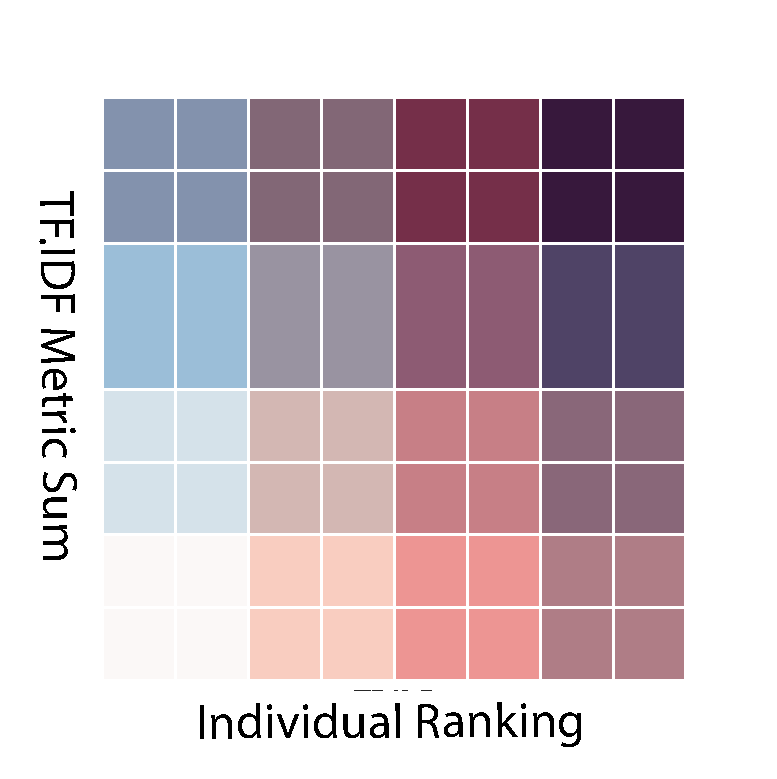
\includegraphics[width=0.4\textwidth,angle=45]{figures_c3/mlpregressor/cbar.pdf}
        \caption{ \textbf{The bivariate colourplot key.} }
        \label{fig:cmap}
\end{figure}


\subsubsection{Individual Categories}
Individual categories are split between traditional metrics and graph centrality metrics. To represent the importance of a species the following values may be extracted through the use of a simple box model:

\begin{itemize}
\item[-] \textbf{Concentration} - This describes the abundance of a species within the atmosphere. 
\item[-] \textbf{Net Flux} - This describes the rate of net (absolute) change of concentration over time for a species. 
\item[-] \textbf{Absolute Flux} - Some species may have a large flux going through them (production and loss), resulting in a small net flux. This sums the production and loss fluxes. 
\item[-] \textbf{Influence} - Influence is the total magnitude of an effect that changing a species concentration by 1\% would have on other species within the network. Since the graph is generated using the Jacobian matrix, an alternative method for calculating this can be by calculating the total out-degree of a node.  
\end{itemize}



The importance of a species is then compared through the use of three of the most common centrality metrics. These are:


\begin{itemize}
\item[-] \textbf{Centrality} - This describes how easily information from one node can be disseminated to all other nodes. 
\item[-] \textbf{Betweenness} - This describes the number of shortest paths (fastest fluxes/greatest influences) that are routed between nodes adjacent to our chosen node. Species with a high betweenness hold a brokering position, and can act as a bottleneck between different groups of chemistry. 
\item[-] \textbf{PageRank} - PageRank looks at the flow in a system. It ranks nodes not only on the number of species it reacts with, but also the importance of the species it has reacted with.

\end{itemize}

Finally the `Metric Sum' is the sum of all the metric values scaled between 1 and zero (the mean).

\subsection{Senario Analysis}

\begin{figure}[H]
     \centering
         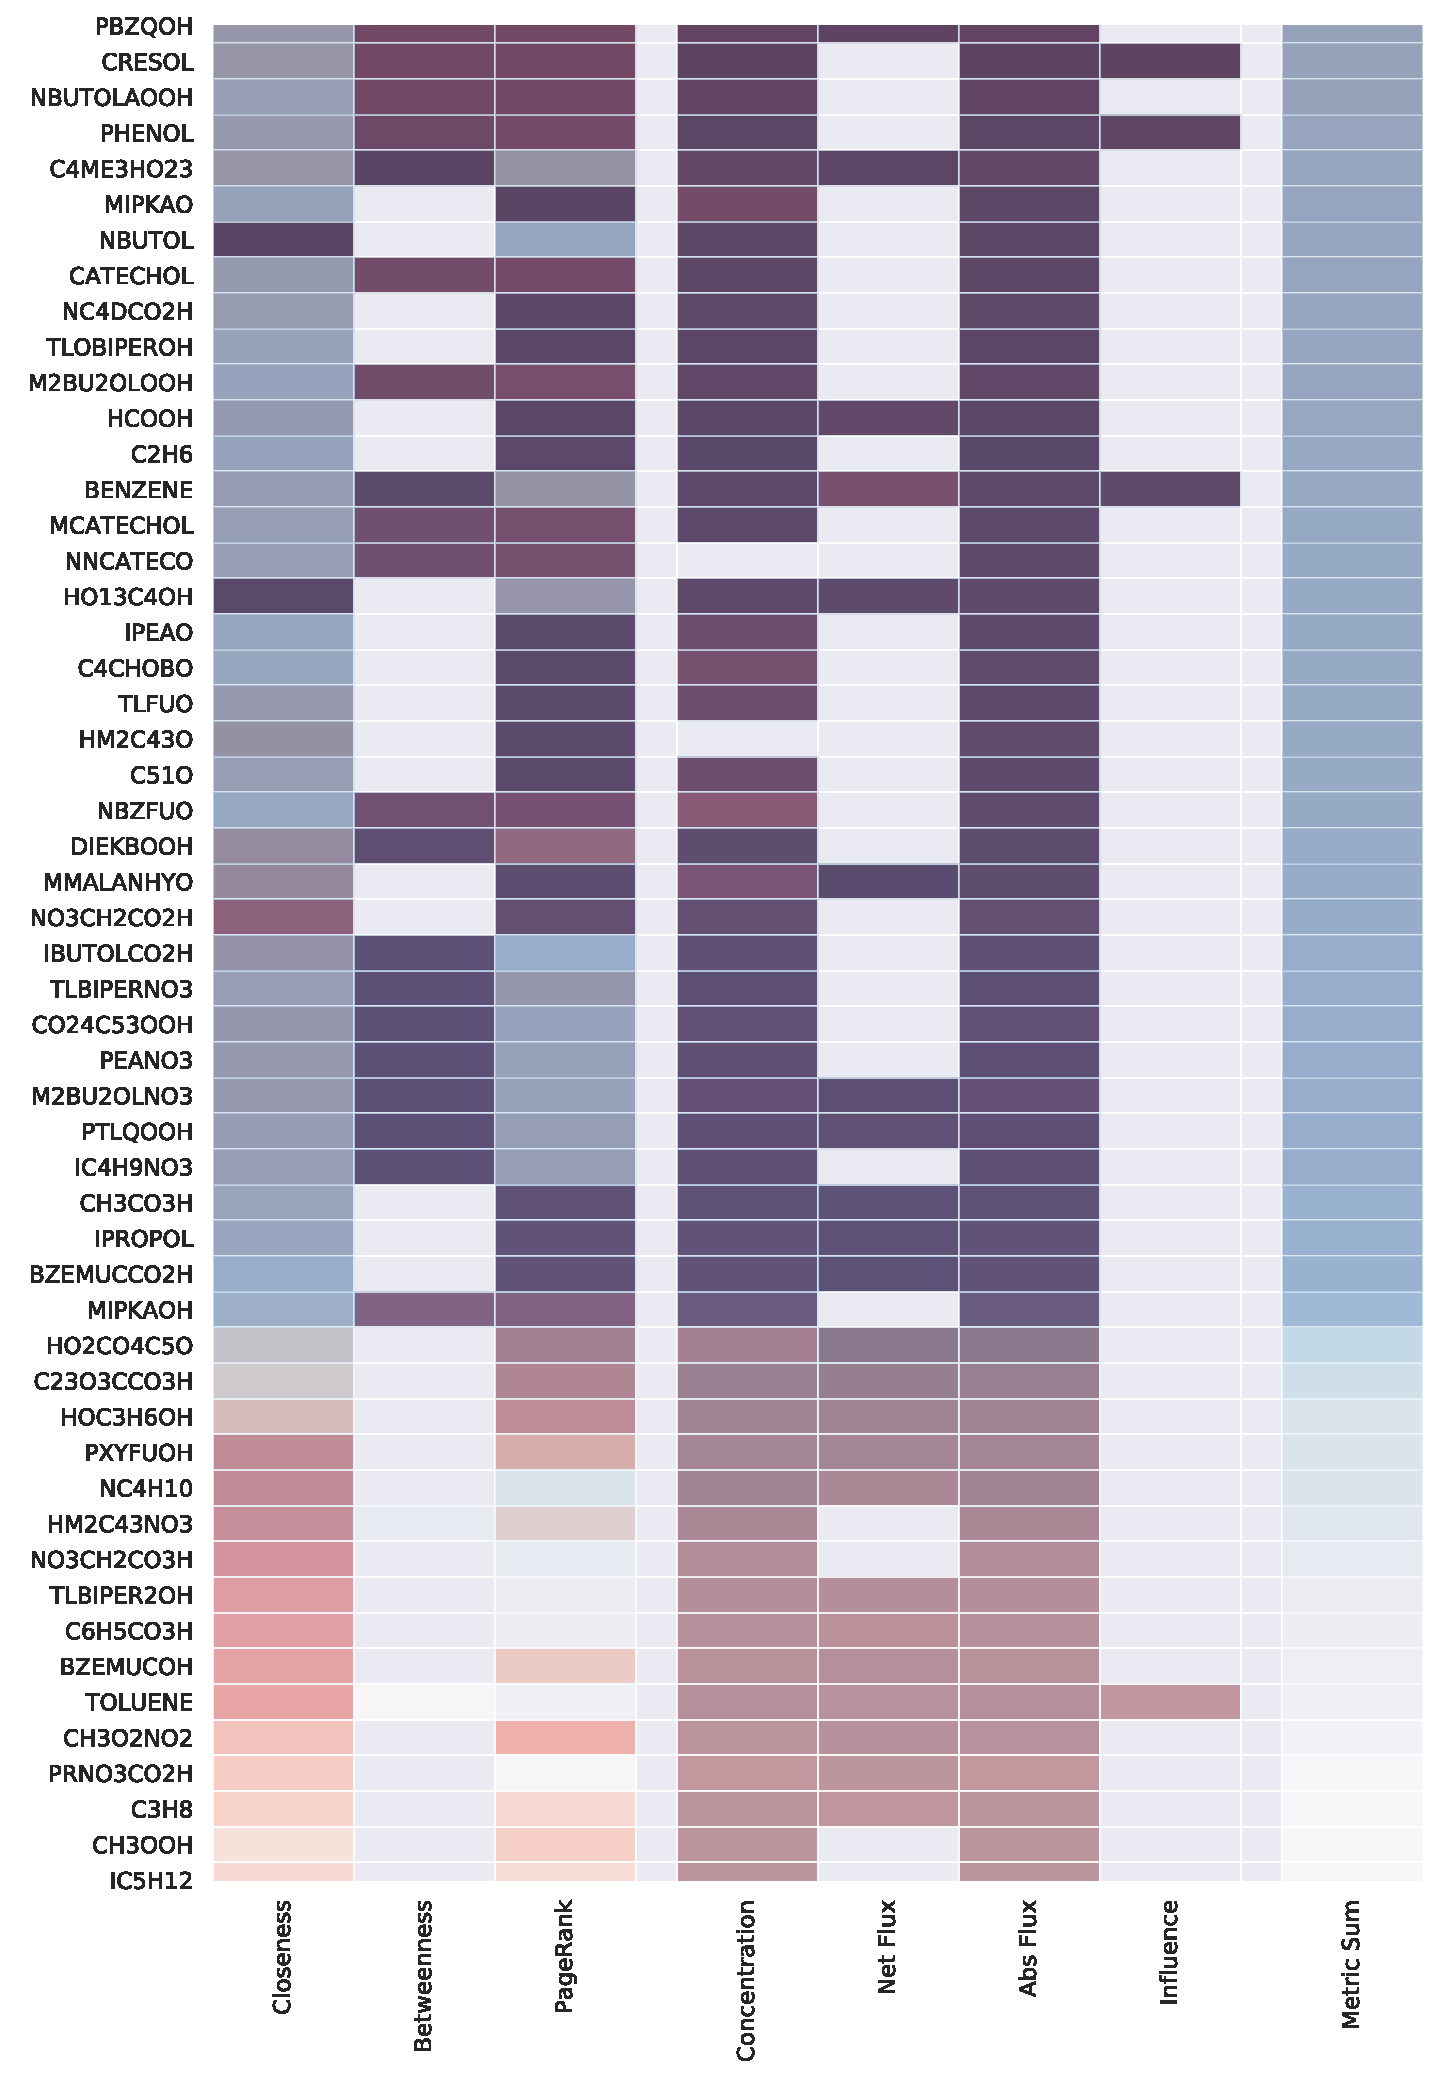
\includegraphics[width=\textwidth]{figures_c3/mlpregressor/cape_CapeVerde.pdf}
        \caption{ \textbf{A bivariate heatmap comparison of Cape Verde.} }
        \label{fig:idf}
\end{figure}

\begin{figure}[H]
     \centering
         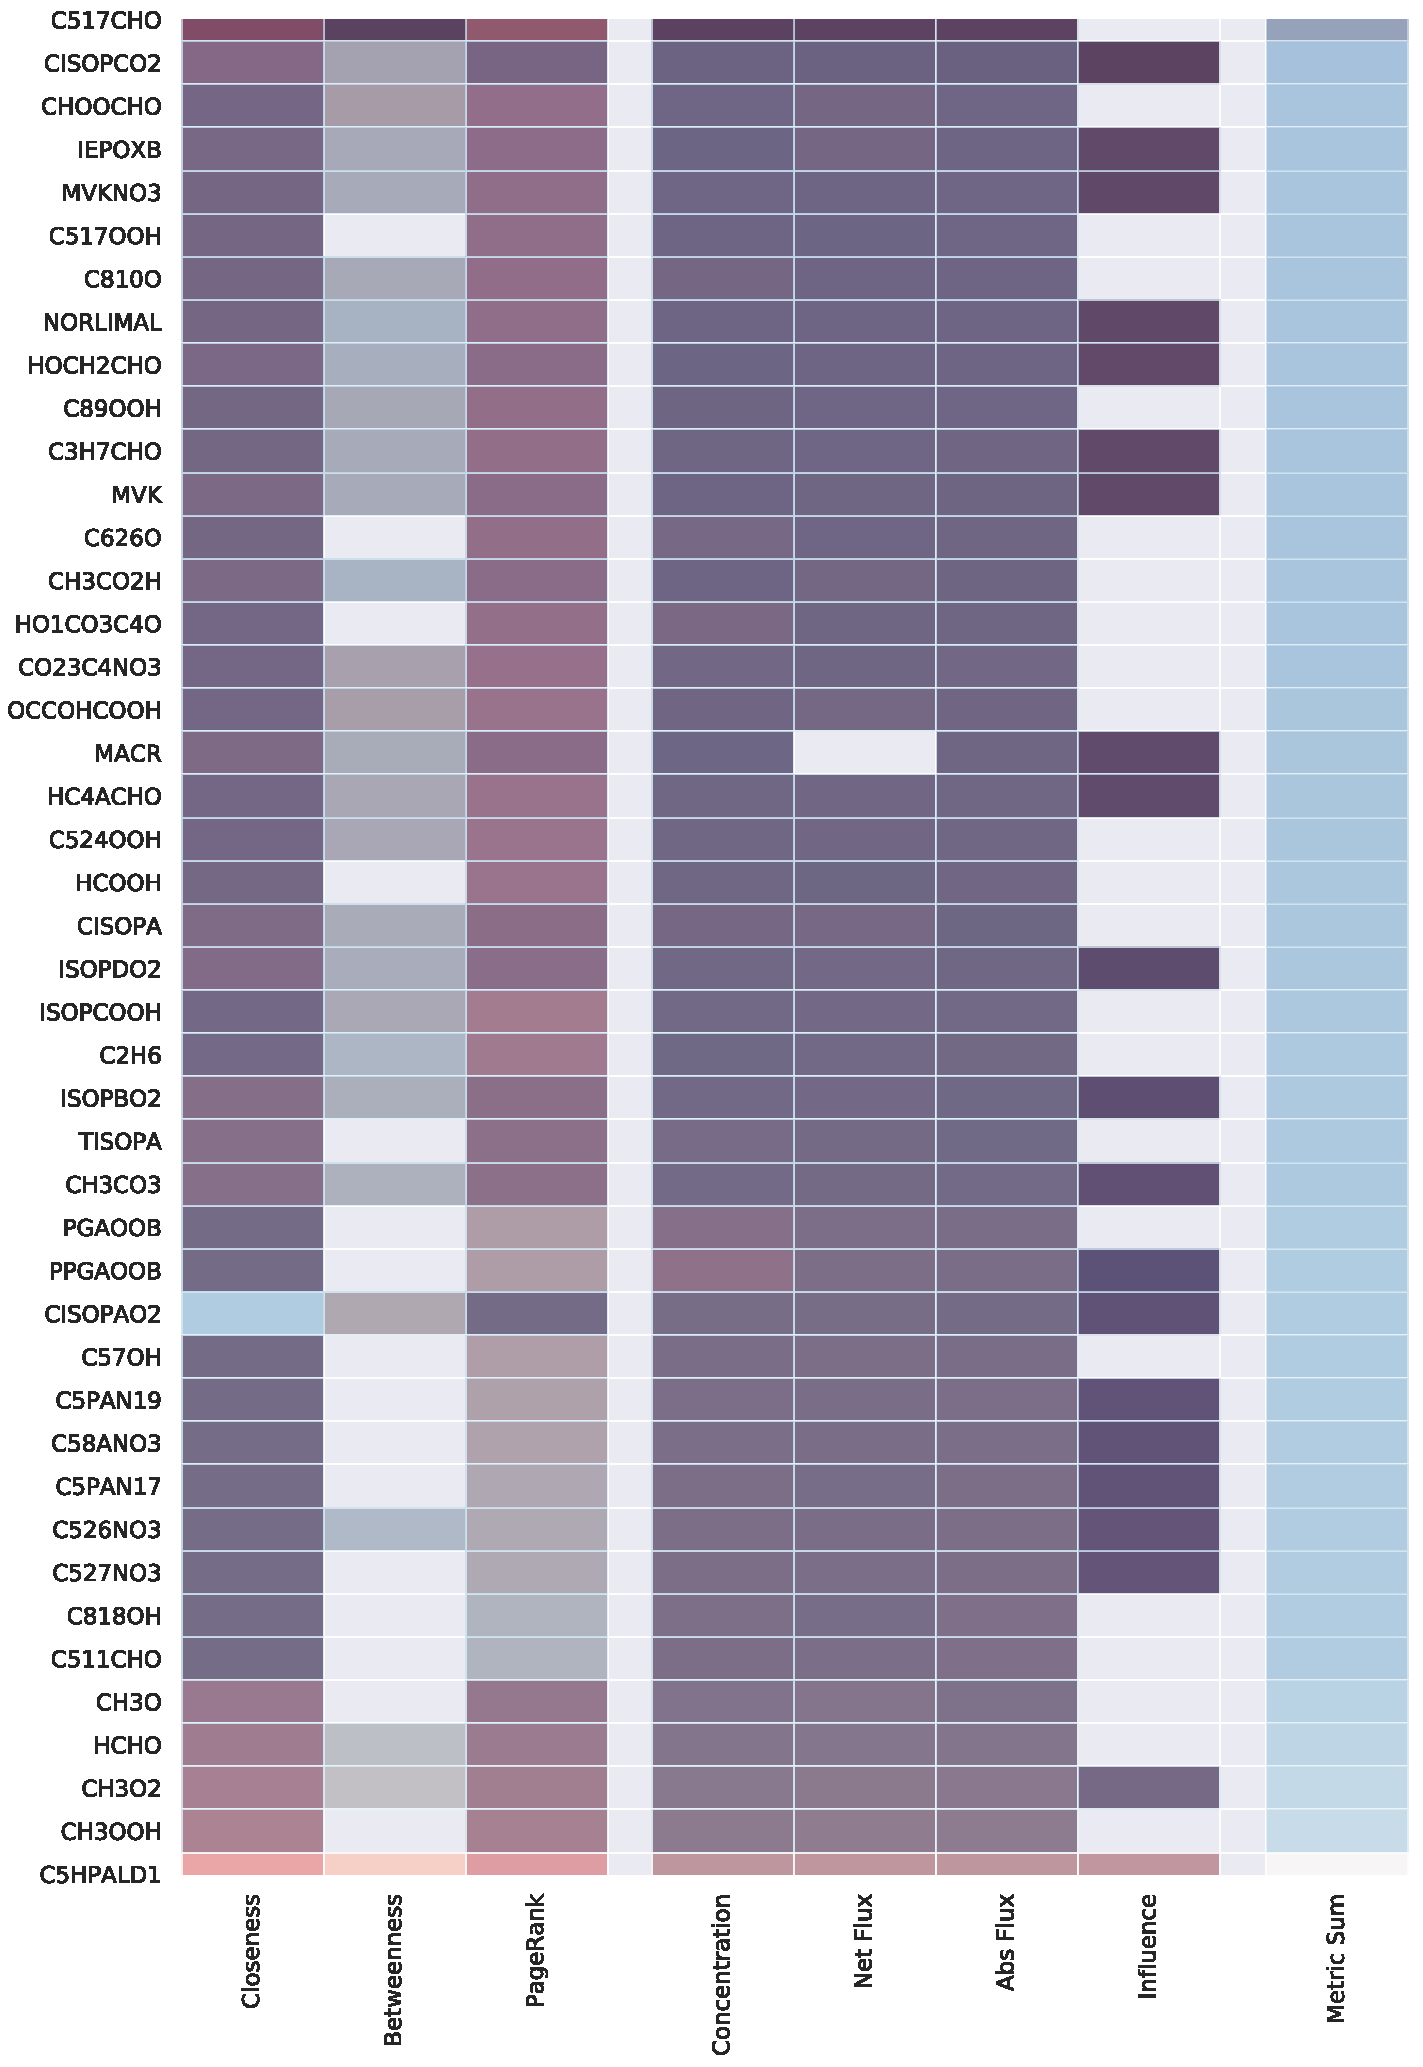
\includegraphics[width=\textwidth]{figures_c3/mlpregressor/op3_Borneo.pdf}
        \caption{ \textbf{A bivariate heatmap comparison of Borneo.} }
        \label{fig:idf}
\end{figure}

\begin{figure}[H]
     \centering
         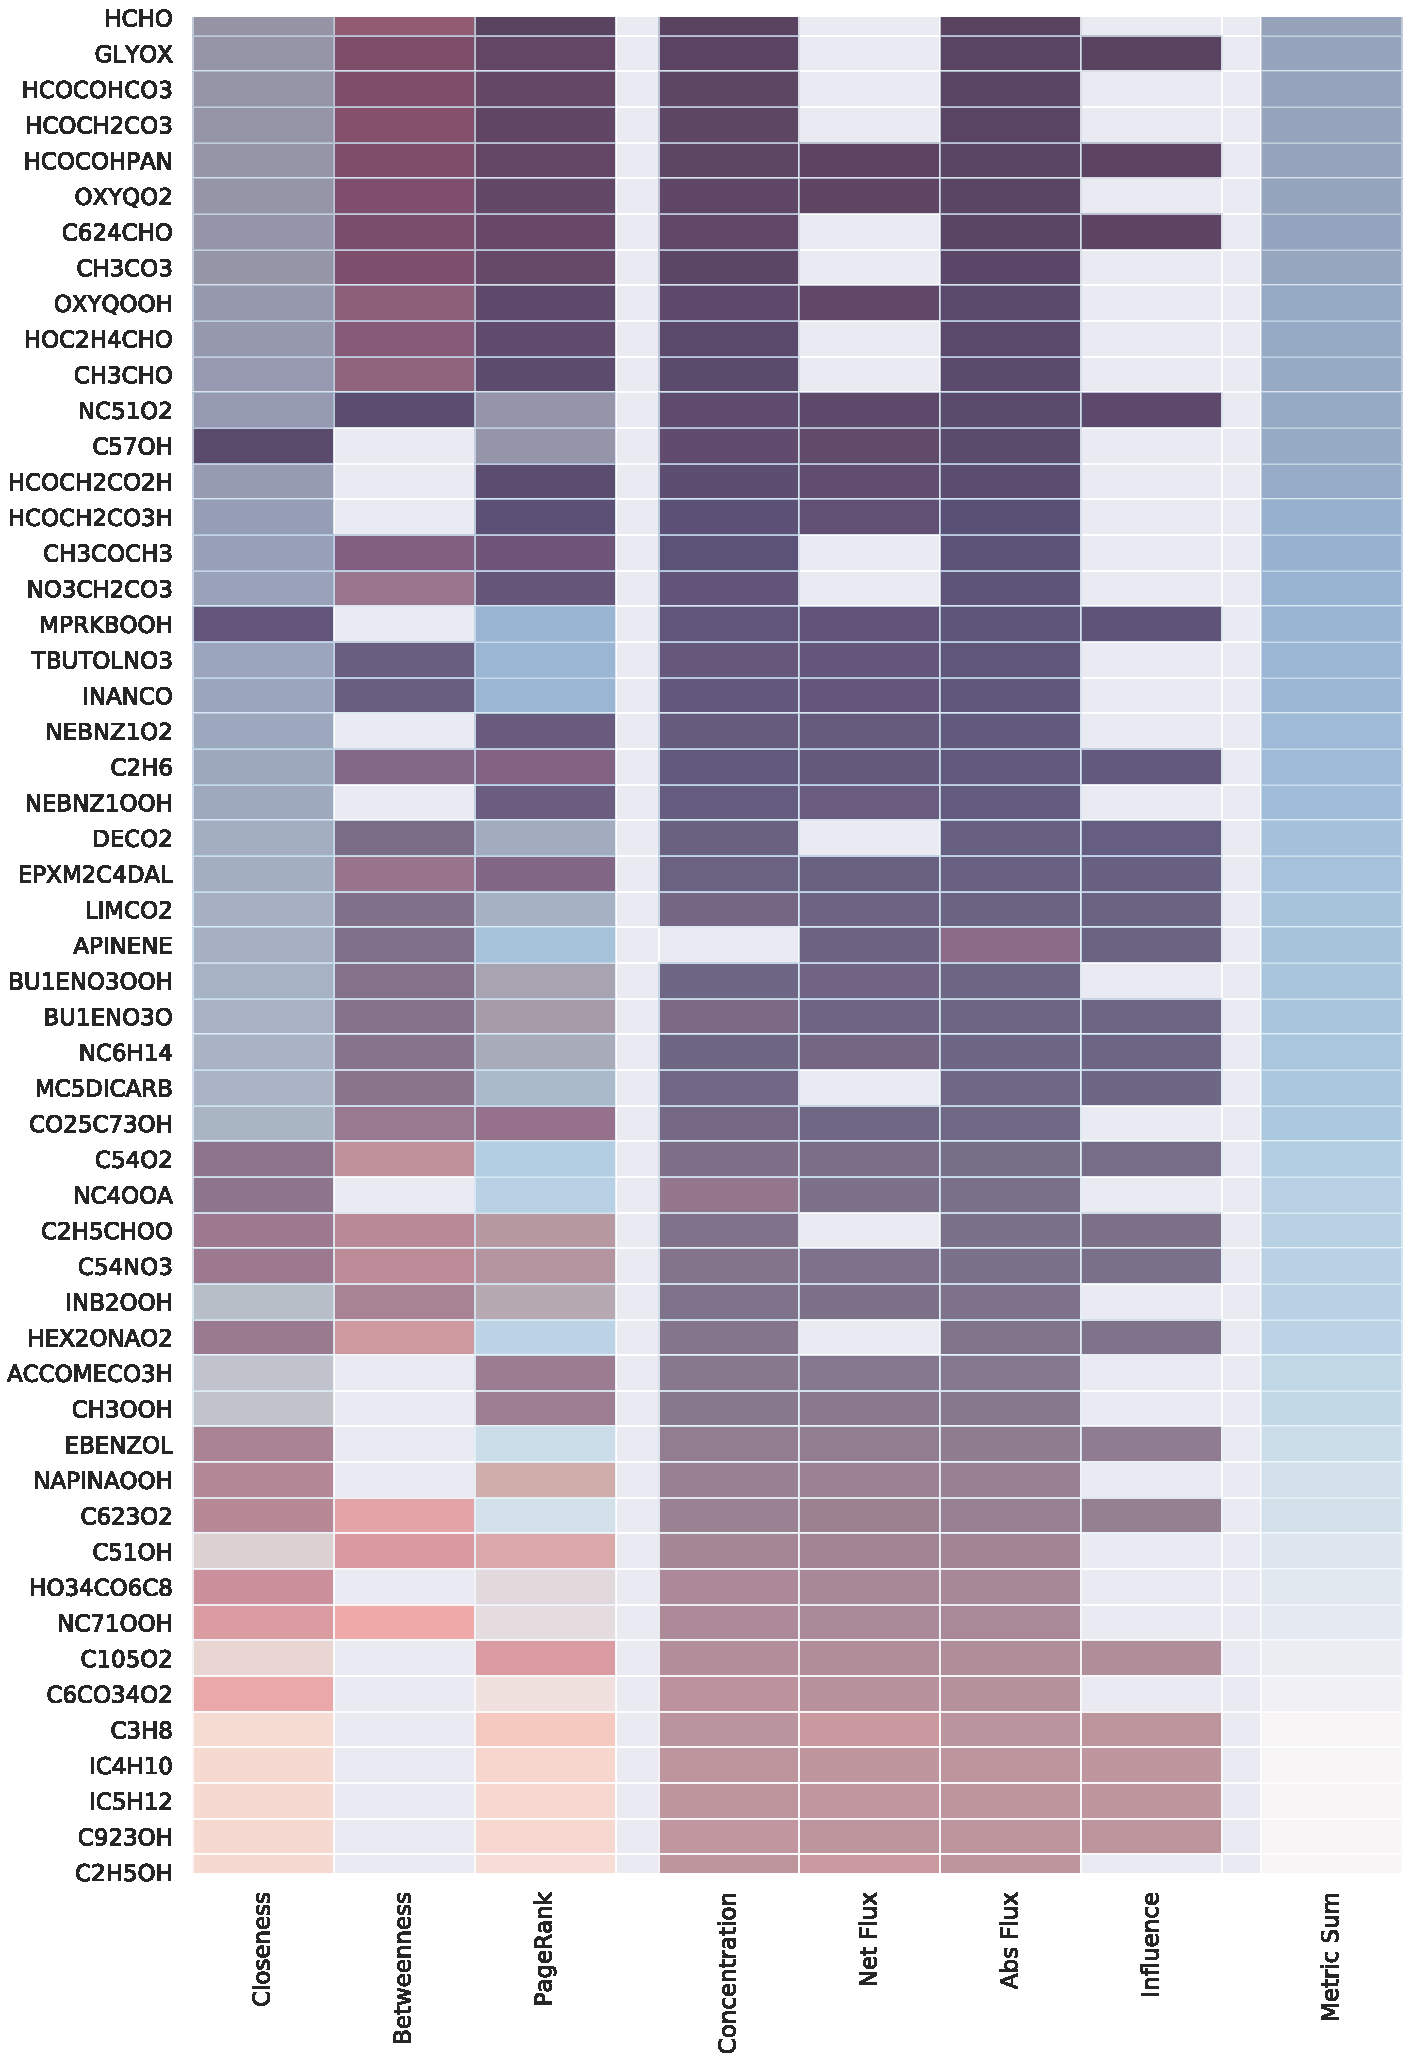
\includegraphics[width=\textwidth]{figures_c3/mlpregressor/clfo_London.pdf}
        \caption{ \textbf{A bivariate heatmap comparison of London.} }
        \label{fig:idf}
\end{figure}

\begin{figure}[H]
     \centering
         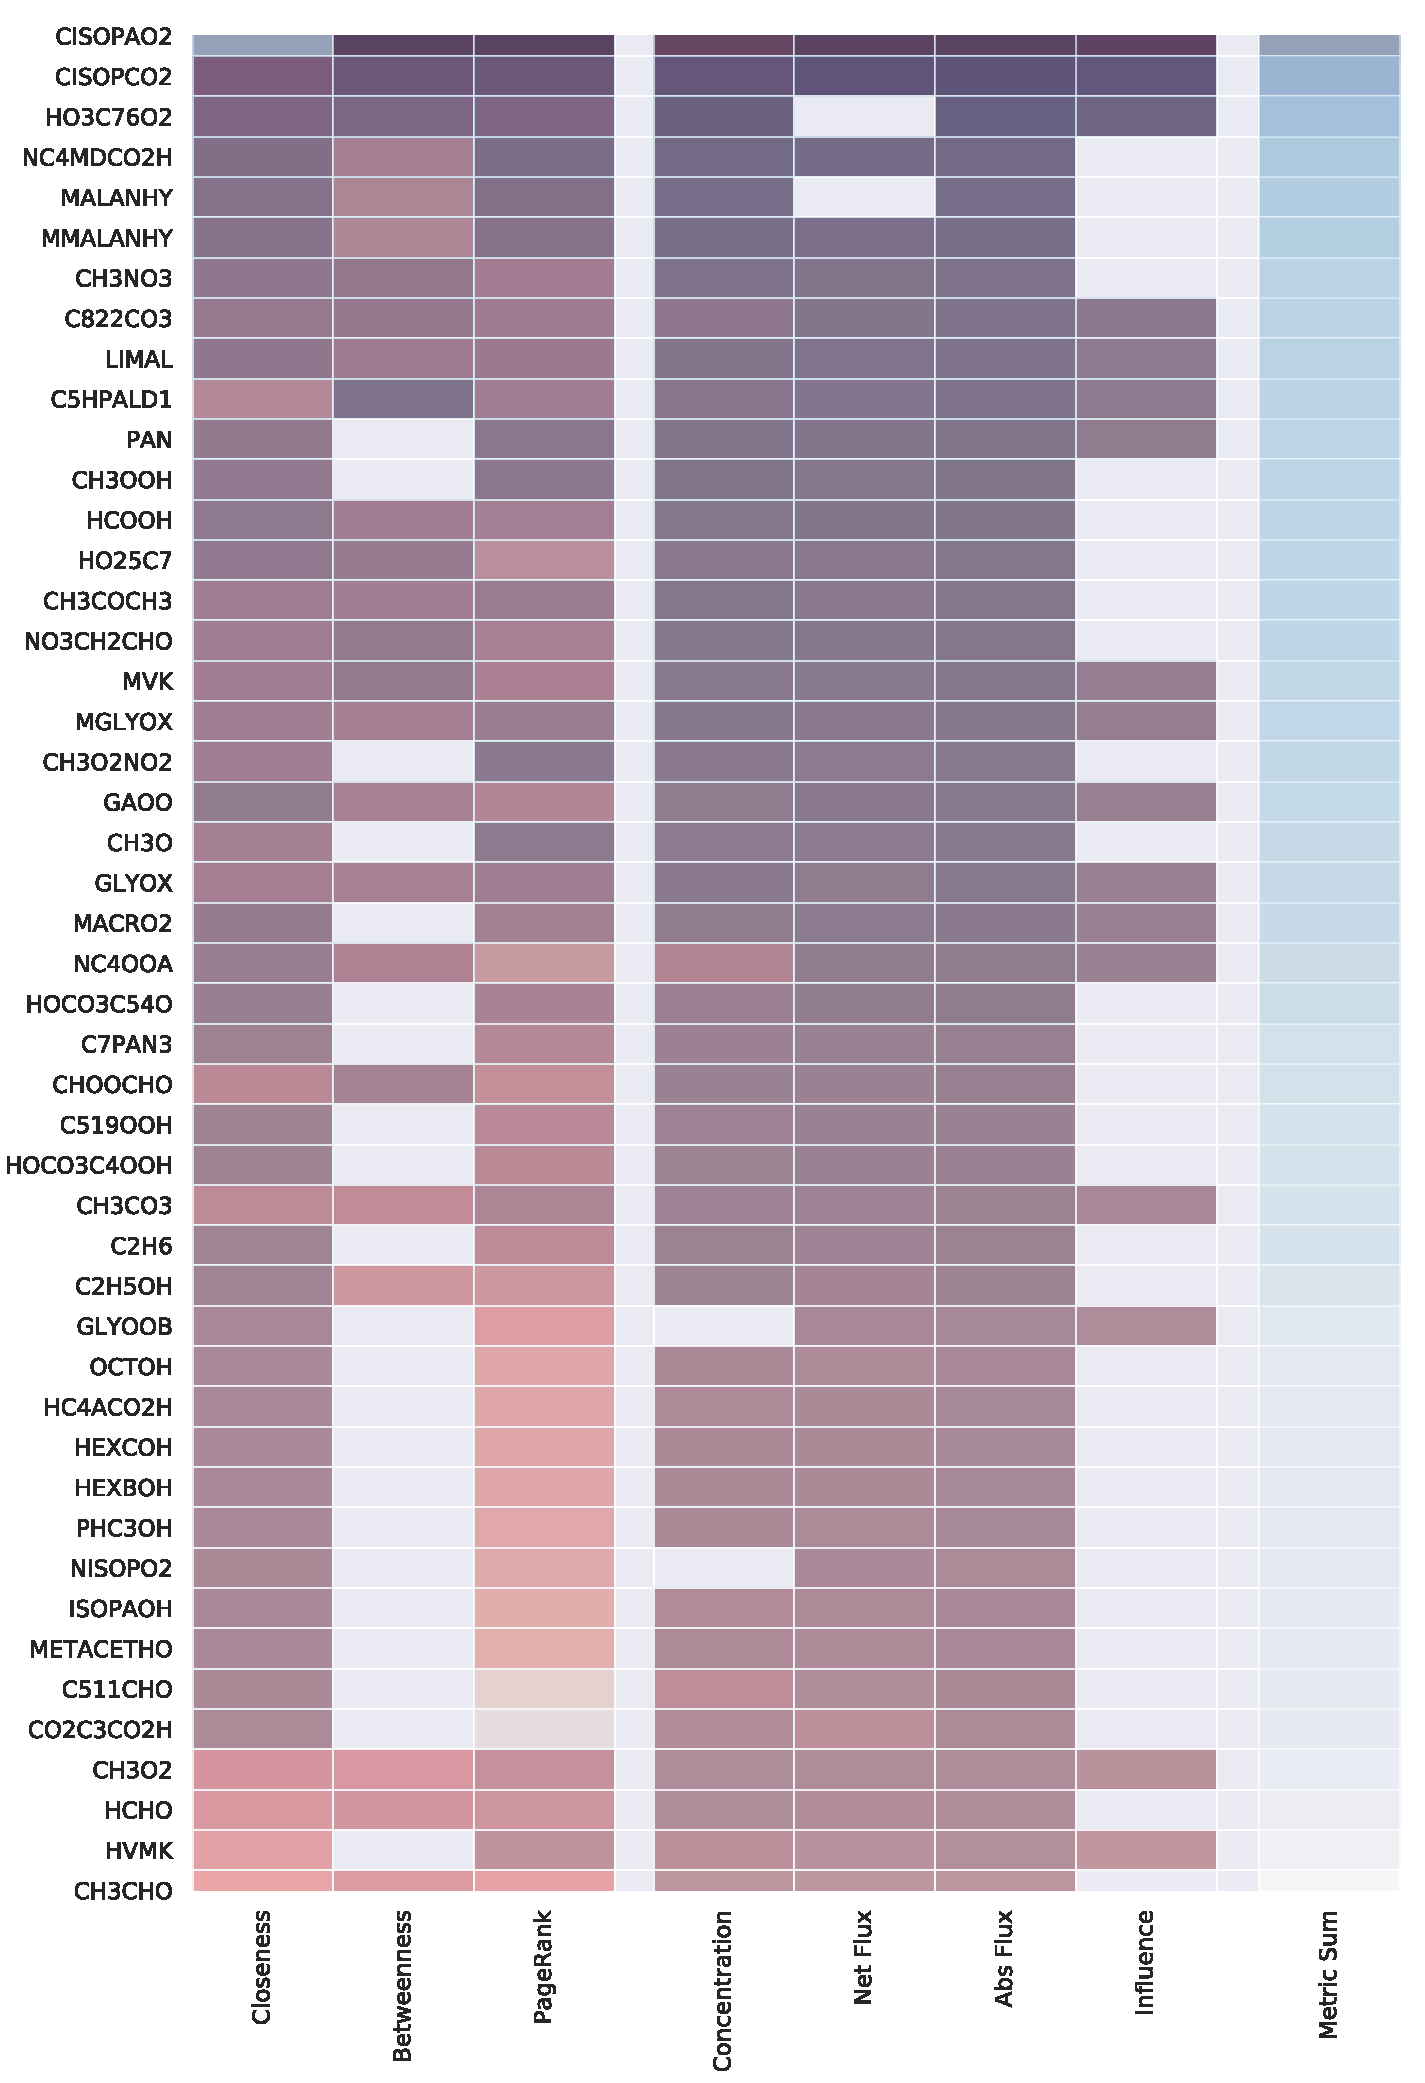
\includegraphics[width=\textwidth]{figures_c3/mlpregressor/aphh_Beijing.pdf}
        \caption{ \textbf{A bivariate heatmap comparison of Beijing.} }
        \label{fig:idf}
\end{figure}

\section{Calculating production sensetivity using personalised page rank.}

\autoref{fig:prtrad}\autoref{fig:pradj}



% http://sibiu.cs.vt.edu/eprints/id/eprint/282/1/Sandu_2003_KPPSEN1.pdf
% The adjoint modeling is presented as an ecient tool to evaluate the sensitivity
% of a scalar response function with respect to the initial conditions and model parameters. In addition,
% sensitivity with respect to time dependent model parameters may be obtained through a single backward
% integration of the adjoint model

\begin{figure}[H]
    \centering
\begin{subfigure}{.9\textwidth}
  \centering
  \includegraphics[width=\textwidth]{figures_c3/traditional.pdf}
  \label{fig:prtrad}
  \caption{Traditional Influence Graph}
\end{subfigure}

\begin{subfigure}{.9\textwidth }
  \centering
  \includegraphics[width=\textwidth]{figures_c3/adjoint.pdf}
  \label{fig:pradj}
  \caption{Reversed-link (adjoint) influence graph}
\end{subfigure}

\caption{\textbf{Link reversal of the Jacobian Sensetivity matrix graph results in a graph of the Adjoint.} Showing how in changing the direction of the links in a graph is equivalent to applying the transpose to an adjacency matrix (right). In the case of a Jacobian based graph, this is analogous to using the adjoint to propagate the model back in time - something that can be used to identify the influence upon a species with a model.}
\end{figure}




\subsection{Testing}
Borneo


As with all scintific processes, it is importatnt to first test the algorithm on a small, comprehensible example. To do this we start with the creation of \ch{ch2oo}. This is a direct product of isoprene. In tracing back all the precursors the mechanism for its creation can be described as: 

\begin{equation}
    \ce{O3 + C5H8 ->[\kappa] CH2OOE}+(MACR\ or\ MVK)\\
    \ce{CH2OOE -> [\kappa_{dec}] CH2OO}
\end{equation}

In traversing the adjoint/reversed graph, this presenets a singe `shortest path' between the product and its precursor. This creates for a base test for the algorithm. The PageRank algorithm is now run with a personalisation vector consisting with an value of 1000000 for the species of interest and -1 for all others. A damping factor value of 0.01 is also used for the algorithm. 

As \ce{CH2OOE} only has one precursor ($\alpha$-pinene) the initial test is done on this. From this the identification of isoprene as a source is sucessful, although since the algorithm is performed on the whole network, there are results for a number of additional species, \autoref{tab:ch2ooe}. This is because page rank works on using teleporation to change between items in the evolution of the system. With the design of the personalisation vector, these values will however be significantly smaller than any containing useful results. 


\begin{table}[H]
    \begin{tabular}{lr}
\toprule
{} &             1 \\
0       &               \\
\midrule
\ch{C5H8}    &  9.920000e-03 \\
\ch{CH2OOE}  &  9.920000e-01 \\
\ch{C816O}   & -9.990000e-07 \\
\ch{NC101CO} & -9.990000e-07 \\
\ch{C926OH}  & -9.990000e-07 \\
\bottomrule
\end{tabular}
\caption{A reversed graph Page Rank test with \ce{C5H8 + O3 -> CH2OOE} as the only reaction.}
\label{tab:ch2ooe}
\end{table} 

Next we apply the same methodology to \ce{CH2OO}. This creates the graph in \autoref{fig:prtest0}. Here it is seen that \ce{CH2OO} is directly dependant on the radicals \ce{CH2OO[F,B,C,G,A]}, and \ce{CH2OOE}. This is then dependant on Isoprene, which then has a range of dependancies with all have precursors of their own (not shown). 


\begin{figure}[H]
  \centering
  \includegraphics[width=\textwidth]{figures_c3/prtest0.png}

  

\caption{\textbf{The reversed subgraph between Isoprene, \ce{CH2OOE} and \ce{CH2OO}.} This is a subgraph of the afforementioned species, showing them and their neighbours. Here the arrows point towards a species precursor. }
\label{fig:prtest0}
\end{figure}

\begin{table}[H]
    \begin{tabular}{lr}
    \toprule
    {} &         1 \\
    0          &           \\
    \midrule
    CH2OO      &  0.992000 \\
    CH2OOE     &  0.001670 \\
    CH2OOF     &  0.001660 \\
    CH2OOG     &  0.001660 \\
    CH2OOA     &  0.001660 \\
    CH2OOC     &  0.001640 \\
    CH2OOB     &  0.001640 \\
    C5H8       &  0.000016 \\
    MACR       &  0.000016 \\
    C2H4       &  0.000007 \\
    HMACR      &  0.000007 \\
    ISOP34NO3  &  0.000005 \\
    ME3BU3ECHO &  0.000005 \\
    ISOPDNO3   &  0.000004 \\
    C622CHO    &  0.000002 \\
    C624CHO    &  0.000002 \\
    C518CHO    &  0.000002 \\
    C729CHO    &  0.000002 \\
    LIMAL      &  0.000002 \\
    C3H6       &  0.000001 \\
    BUT1ENE    &  0.000001 \\
    PE4E2CO    &  0.000001 \\
    MVK        &  0.000001 \\
    MVKOH      &  0.000001 \\
    ISOPBNO3   &  0.000001 \\
    ACR        &  0.000001 \\
    \bottomrule
    \end{tabular}

\caption{A reversed graph Page Rank test with \ce{C5H8 + O3 -> CH2OOE} as the only reaction.}
\label{tab:ch2oo}
\end{table} 





\newpage

\bibliographystyle{apalike}
\bibliography{centrality,metric}
% \bibliographystyle{unsrt}




\end{document}
